%-------------------------------------------------------------------------------
% Copyright (c) 2015-2016 University of Luxembourg.
% All rights reserved. This program and the accompanying materials
% are made available under the terms of the Eclipse Public License v1.0
% which accompanies this distribution, and is available at
% http://www.eclipse.org/legal/epl-v10.html
% 
% Contributors:
%     Alfredo Capozucca - initial writingg
%     
%-------------------------------------------------------------------------------
%%%%%%%%%%%%%%%%%%%%%%%%%%%%%%%%%%%%%%%%%%%%%%%%%%
\PassOptionsToPackage{usenames,svgnames,table}{xcolor}
\documentclass[graybox,envcountchap,sectrefs]{./../lu.uni.lassy.excalibur.standard.report.libraries/styles/svmono}
%%%%%%%%%%%%%%%%%%%%%%%%%%%%%%%%%%%%%%%%%%%%%%%%%%
%%% DO NOT CHANGE THE ORDER
\usepackage{./../lu.uni.lassy.excalibur.standard.report.libraries/styles/style-messir-common}
\usepackage{./../lu.uni.lassy.excalibur.standard.report.libraries/styles/style-messir-report-post}
\usepackage{breakurl}    
%--------------------------------------------
 
% DOCUMENT BEGIN
%--------------------------------------------
\begin{document}
%-------------------------------------------------------------------------------
 
\newgeometry{textwidth=17cm,textheight=23.7cm} 
 
\definecolor{lightgray}{RGB}{201,201,201}
\definecolor{lightred}{RGB}{250,112,97}
\definecolor{lightgreen}{RGB}{179,250,140}

\definecolor{msrtextcl}{RGB}{0,0,0}
\definecolor{msrkeycl}{RGB}{127,0,85}
\definecolor{msrcmtcl}{RGB}{201,201,201}
\definecolor{keywordcolor}{RGB}{30,144,255}

\definecolor{aqua_blue}{RGB}{0,139,145}
\definecolor{dark_green}{RGB}{0,128,0}
\definecolor{dark_blue}{RGB}{45,45,138}

\definecolor{msrcolor01}{rgb}{0.96,0.59,0.48}
\definecolor{msrcolor02}{rgb}{1.00,0.97,0.60}
\definecolor{msrcolor03}{rgb}{0.51,0.79,0.61}
\definecolor{msrcolor04}{rgb}{0.43,0.81,0.96}
\definecolor{msrcolor05}{rgb}{0.52,0.58,0.79}
\definecolor{msrcolor06}{rgb}{0.96,0.61,0.76}
\definecolor{msrcolor07}{rgb}{0.98,0.68,0.51}
\definecolor{msrcolor08}{rgb}{0.77,0.88,0.61}
\definecolor{msrcolor09}{rgb}{0.49,0.66,0.85}
\definecolor{msrcolor10}{rgb}{0.96,0.60,0.62}
\definecolor{msrcolor11}{rgb}{0.64,0.83,0.61}
\definecolor{msrcolor12}{rgb}{0.63,0.53,0.75}
\definecolor{msrcolor13}{rgb}{0.99,0.78,0.54}
\definecolor{msrcolor14}{rgb}{0.53,0.51,0.74}
\definecolor{msrcolor15}{rgb}{0.48,0.80,0.79}
\definecolor{msrcolor16}{rgb}{0.74,0.55,0.75}
\definecolor{msrcolor17}{rgb}{0.90,0.79,0.08}
\definecolor{msrcolor18}{rgb}{1.00,1.00,0.00}
\definecolor{msrcolor19}{rgb}{1.00,0.00,0.50}

\definecolor{sepcolor000000}{rgb}{0, 0, 0}
\definecolor{sepcolor101010}{rgb}{0.10, 0.10, 0.10}
\definecolor{sepcolor202020}{rgb}{0.20, 0.20, 0.20}
\definecolor{sepcolor303030}{rgb}{0.30, 0.30, 0.30}
\definecolor{sepcolor404040}{rgb}{0.10, 0.10, 0.10}
\definecolor{sepcolor505050}{rgb}{0,1,.5}
\definecolor{sepcolor907908}{rgb}{0,1,.5}

\definecolor{sepregioncolor01}{rgb}{0.00,0.66,0.00}
\definecolor{sepregioncolor02}{rgb}{1.00,1.00,0.00}
\definecolor{sepregioncolor03}{rgb}{1.00,0.97,0.60}
\definecolor{sepregioncolor04}{rgb}{0.64,0.83,0.61}
\definecolor{sepregioncolor05}{rgb}{0.95,0.36,0.00}
\definecolor{sepregioncolor06}{rgb}{0.90,0.79,0.08}
\definecolor{sepregioncolor07}{rgb}{0.63,0.53,0.75}
\definecolor{sepregioncolor08}{rgb}{0.99,0.78,0.54}
\definecolor{sepregioncolor09}{rgb}{0.96,0.61,0.76}
\definecolor{sepregioncolor10}{rgb}{1.00,0.00,0.50}

\colorlet{msrcolorbrown}{red!40!black!80}


% Messir General
%----------------------------------------------------------

% quotePosition + quoteWidth + quotefillColor + quoteElement + quotedElement + allImageScale
\newcommand{\msrcallouted}[6]{
\scalebox{#1}{\parbox{\linewidth}{
  \begin{tikzpicture}
      \node [rectangle callout,callout relative pointer={#4},text width=#5,fill=#6,rounded corners] (tmpcall) at (0,0) {#3};
      \node at (tmpcall.pointer){#2};
  \end{tikzpicture}
}}
}

% Vresion wihtout scaling the quoted text
\pgfkeys{%
    /calloutquote/.cd,
    width/.code                   =  {\def\calloutquotewidth{#1}},
    position/.code                =  {\def\calloutquotepos{#1}}, 
    author/.code                  =  {\def\calloutquoteauthor{#1}},
    /calloutquote/.unknown/.code   =  {\let\searchname=\pgfkeyscurrentname
                                 \pgfkeysalso{\searchname/.try=#1,
    /tikz/\searchname/.retry=#1},\pgfkeysalso{\searchname/.try=#1,
                                  /pgf/\searchname/.retry=#1}}
                            }  

\newcommand\calloutquote[2][]{%
  \pgfqkeys{/calloutquote}{#1}
  \node [rectangle callout,callout relative pointer={\calloutquotepos},text width=\calloutquotewidth,/calloutquote/.cd,#1] (tmpcall) at (0,0) {#2};
  \node at (tmpcall.pointer){\calloutquoteauthor};    
}  
%----------------------------------------------------------
\newcommand{\msrTalkRD}[6]{
\freeblock{5}{#1}{#2}{
\begin{figure}
  \centering
  \includegraphics[width=#5]{images/various/descartes.pdf} 
\end{figure}
}
\freeblock{5}{#3}{#4}{
\scriptsize
\textit{#6}
}
}
\newcommand{\msrTalkGB}[6]{
\freeblock{5}{#1}{#2}{
\begin{figure}
  \centering
  \includegraphics[width=#5]{images/various/graham-bell.pdf} 
\end{figure}
}
\freeblock{5}{#3}{#4}{
\scriptsize
\textit{#6}
}
}
%----------------------------------------------------------

\newcommand{\msrQuestionSlide}[1]{
\begin{frame}[fragile]
\freeblock{5}{1}{4}{
\begin{figure}
  \centering
  \includegraphics[width=3cm]{images/various/3d-man-question-sit.pdf}
\end{figure}
}
\freeblock{10}{5}{3}{
\Large
\msrtxtclb{red}{\textit{#1}}
}
\end{frame}
}

%%%%%%%%%%%%%%%%%%%%%%%%%%%%%%%%%%%%%%%%%%%%%%%%%%

\DeclareRobustCommand{\msrfigure}[4]{
\begin{figure}[htbp]
%\centering
\scalebox{#1}{
{\begin{minipage}[c]{\linewidth}
\centering
#2
\end{minipage}
}}
\ifthenelse{\equal{#4}{}}
             {}
             {\caption{#4}}
\label{#3}
\end{figure}
}

\newcommand{\semitransp}[2][30]{\color{fg!#1}#2}
\newcommand*{\msrtechfont}{\fontfamily{ptm}\selectfont}

\DeclareRobustCommand{\msruml}{{\msrtechfont UML}~}
\DeclareRobustCommand{\msrocl}{{\msrtechfont OCL}~}
\DeclareRobustCommand{\msromg}{{\msrtechfont OMG}~}
\DeclareRobustCommand{\msrxtext}{{\msrtechfont Xtext}~}
\DeclareRobustCommand{\msremf}{{\msrtechfont EMF}~}
\DeclareRobustCommand{\msrcm}{\msrcode{{Concept Model}}~}

\DeclareRobustCommand{\msrapache}{{\msrtechfont Apache}~}
\DeclareRobustCommand{\msratlassian}{{\msrtechfont Atlassian}~}
\DeclareRobustCommand{\msrbamboo}{{\msrtechfont Bamboo}~}
\DeclareRobustCommand{\msrconfluence}{{\msrtechfont Confluence}~}
\DeclareRobustCommand{\msreclemma}{{\msrtechfont EclEmma}~}
\DeclareRobustCommand{\msreclipse}{{\msrtechfont Eclipse}~}
\DeclareRobustCommand{\msrsql}{{\msrtechfont SQL}~}
\DeclareRobustCommand{\msrjava}{{\msrtechfont Java}~}
\DeclareRobustCommand{\msrjavafx}{{\msrtechfont JavaFx}~}
\DeclareRobustCommand{\msrjira}{{\msrtechfont JIRA}~}
\DeclareRobustCommand{\msrjunit}{{\msrtechfont JUnit}~}
\DeclareRobustCommand{\msrlatex}{{\msrtechfont Latex}~}
\DeclareRobustCommand{\msrmaven}{{\msrtechfont Maven}~}
\DeclareRobustCommand{\msrmysql}{{\msrtechfont MySQL}~}
\DeclareRobustCommand{\msrocl}{{\msrtechfont OCL}~}
\DeclareRobustCommand{\msrpdf}{{\msrtechfont PDF}~} 
\DeclareRobustCommand{\msrsirius}{{\msrtechfont Sirius}~} 
\DeclareRobustCommand{\msrsvn}{{\msrtechfont SubVersioN}~}
\DeclareRobustCommand{\msrswtbot}{{\msrtechfont SWTbot}~}
\DeclareRobustCommand{\msrxtext}{{\msrtechfont Xtext}~} 

 
\DeclareRobustCommand{\msrmessirmeth}{{\msrmessir}~methodology~}
\newcommand{\msrglsstyle}[1]{\emph{#1}}
\DeclareRobustCommand{\msrucname}[1]{\msrcode{\underline{#1}}}

% Verify macro since creates .toc errors
%\DeclareRobustCommand{\msrcode}[1]{{\normalfont\fontfamily{pcrr}\selectfont #1}}
%\DeclareRobustCommand{\msrcode}[1]{{\normalfont\fontfamily{cmvtt}\selectfont #1}}
\DeclareRobustCommand{\msrcode}[1]{{\protect\ \ttfamily \hyphenchar\font=`\- #1}}

% Messir Lexique
\DeclareRobustCommand{\msrbool}{\msrcode{{\emph Boolean}}~}
\DeclareRobustCommand{\msrint}{\msrcode{{\emph Integer}}~}
\DeclareRobustCommand{\msrreal}{\msrcode{{\emph Real}}~}
\DeclareRobustCommand{\msrstring}{\msrcode{{\emph String}}~}
\DeclareRobustCommand{\msrenum}{\msrcode{{\emph enumeration}}~}
\DeclareRobustCommand{\msrenums}{\msrcode{{\emph enumerations}}~}

% Messir Analysis
\DeclareRobustCommand{\msrsysop}{\emph{system operation}}
\DeclareRobustCommand{\msrsysops}{\emph{system operations}}
\DeclareRobustCommand{\msrsysintpro}{\emph{system interaction protocol}}
\DeclareRobustCommand{\msrbhvmd}{\emph{system operation}}

\newcommand{\msrt}[1]{\textuncl{#1}~}

\DeclareRobustCommand{\msrfont}[1]{\textuncl{#1}}
\DeclareRobustCommand{\msrfontb}[1]{\msrfont{\textbf{#1}}}
\DeclareRobustCommand{\msrfontcl}[1]{\msrfont{{\color{MediumPurple}#1}}}
\DeclareRobustCommand{\msrfontclb}[1]{{\msrfontcl{\textbf{#1}}}}

\DeclareRobustCommand{\msrcl}[1]{{\color{MediumPurple}#1}~}
\DeclareRobustCommand{\msrclb}[1]{{\msrcl{\textbf{#1}}}}

\DeclareRobustCommand{\msrmessir}{\msrfont{Messir}~}
\DeclareRobustCommand{\msrmessirb}{\msrfont{\textbf{Messir}}}
\DeclareRobustCommand{\msrmessircl}{{\color{MediumPurple}\msrmessir}}
\DeclareRobustCommand{\msrmessirclb}{{\color{MediumPurple}\msrmessirb}}

\DeclareRobustCommand{\msrexcalibur}{{\unclfamily Excalibur}~}
\DeclareRobustCommand{\msrexcaliburb}{\msrfont{\textbf{\msrexcalibur}}}
\DeclareRobustCommand{\msrexcaliburcl}{\msrfontcl{\msrexcalibur}}
\DeclareRobustCommand{\msrexcaliburclb}{\msrfontclb{\msrexcalibur}}

\DeclareRobustCommand{\msrmessim}{\msrfont{MesSim}}
\DeclareRobustCommand{\msrmessimb}{\msrfontb{MesSim}}
\DeclareRobustCommand{\msrmessimcl}{\msrfontcl{MesSim}}
\DeclareRobustCommand{\msrmessimclb}{\msrfontclb{MesSim}}

\DeclareRobustCommand{\msrmessam}{\msrfont{MesSam}}
\DeclareRobustCommand{\msrmessamb}{\msrfontb{MesSam}}
\DeclareRobustCommand{\msrmessamcl}{\msrfontcl{MesSam}}
\DeclareRobustCommand{\msrmessamclb}{\msrfontclb{MesSam}}

\DeclareRobustCommand{\msrmevop}{\msrfont{MevoP}~}
\DeclareRobustCommand{\msrmevopb}{\msrfontb{MevoP}~}
\DeclareRobustCommand{\msrmevopcl}{\msrfontcl{MevoP}~}
\DeclareRobustCommand{\msrmevopclb}{\msrfontclb{MevoP}~}

\DeclareRobustCommand{\msrmessep}{\msrfont{Messep}~}
\DeclareRobustCommand{\msrmessepb}{\msrfontb{Messep}~}
\DeclareRobustCommand{\msrmessepcl}{\msrfontcl{Messep}~}
\DeclareRobustCommand{\msrmessepclb}{\msrfontclb{Messep}~}

\DeclareRobustCommand{\msrmessee}{\msrfont{MesSEE}~}
\DeclareRobustCommand{\msrmesseeb}{\msrfontb{MesSEE}~}
\DeclareRobustCommand{\msrmesseecl}{\msrfontcl{MesSEE}~}
\DeclareRobustCommand{\msrmesseeclb}{\msrfontclb{MesSEE}~}

\DeclareRobustCommand{\msrprolog}{{\msrtechfont Prolog}}
\DeclareRobustCommand{\msrmessimb}{\textbf{\msrmessim}}
\DeclareRobustCommand{\msrprologcl}{\textcolor{red}{\msrprolog}}
\DeclareRobustCommand{\msrprologclb}{\textbf{\msrprologcl}}

\DeclareRobustCommand{\msrmcl}{{\footnotesize \msrfont{mcl}}}
\DeclareRobustCommand{\msrmclb}{\msrfontb{\msrmcl}}
\DeclareRobustCommand{\msrmclclb}{\msrfontcl{\msrmclb}}
\DeclareRobustCommand{\msrmclcl}{\msrfontcl{\msrmcl}}

\DeclareRobustCommand{\msrmcltt}{\protect\ \msrmessir Constraint Language~}
\DeclareRobustCommand{\msrmessimtt}{\protect\ \msrmessir Simulator~}
\DeclareRobustCommand{\msrmessamtt}{\protect\ \msrmessir Abstract Machine~}

\DeclareRobustCommand{\generic}{\textbf{\textit{{\color{MediumPurple}generic}}}~} 
\DeclareRobustCommand{\msrhelloworld}{\textbf{\textit{{\color{MediumPurple}HelloWorld}}}~}
\DeclareRobustCommand{\msricrash}{\textbf{\textit{{\color{MediumPurple}iCrash}}}~} 
\DeclareRobustCommand{\msricrashmini}{\textbf{\textit{{\color{MediumPurple}iCrashMini}}}~}  

\DeclareRobustCommand{\msrtxtcl}[2]{{\color{#1}#2}}
\DeclareRobustCommand{\msrtxtclb}[2]{\msrtxtcl{#1}{\textbf{#2}}}


%---------TABLES TEMPLATE--------------

%\rowcolors{2}{gray!20}{}

\newcounter{itemtable}


\newenvironment{usecase}{\begin{longtable}{|p{0.10\textwidth}
p{0.90\textwidth}|} \hline} {\hline \end{longtable}}


\newenvironment{usecaseinstance}{\begin{longtable}{|p{0.05\textwidth}
p{0.95\textwidth}|} \hline}
{\hline \end{longtable}}


\newenvironment{actortable}{
\begin{longtable}{|p{0.10\textwidth} p{0.90\textwidth}|}
\hline \hline}
{\hline \end{longtable}}


\newenvironment{datadictionary}{
\begin{longtable}{|p{0.15\textwidth} p{0.85\textwidth}|}
\hline \hline}
{\hline \end{longtable}}


\newenvironment{associationtypes}{
\begin{longtable}{|p{0.15\textwidth} p{0.85\textwidth}|}
\hline \hline}
{\hline \end{longtable}}


\newenvironment{operationmodel}{
\setcounter{itemtable}{0}
\begin{longtable}{|p{0.10\textwidth} p{0.90\textwidth}|}
\hline \hline}
{\hline \end{longtable}}


\newenvironment{teststepmodel}{
\setcounter{itemtable}{0}
\begin{longtable}{|p{0.10\textwidth}|p{0.90\textwidth}|}
\hline}
{\hline \end{longtable}}


\newcommand*{\myfont}{\fontfamily{phv}\selectfont}


\newcommand\addheading[1]{
\hline
%\multicolumn{2}{|l|}{\cellcolor[gray]{0.9} \textbf{#1}} \\
\multicolumn{2}{|l|}{\textbf{\scshape #1}} \\
\hline \hline
\endfirsthead

\multicolumn{2}{@{}l}{\myfont{\bfseries\itshape{\ldots #1 table
continuation}}}\\
%\hline \hline
%\multicolumn{2}{|l|}{\cellcolor[gray]{0.9} \textbf{#1}}\\
%\hline \hline
\endhead % all the lines above this will be repeated on every page

%\hline \hline
\multicolumn{2}{r@{}}{\myfont{\bfseries\itshape{continues in next page
\ldots}}}\\
\endfoot

\hline
\endlastfoot}

%\multicolumn{2}{|l|}{\cellcolor[gray]{0.8}
\newcommand\addrowheading[1]{
\hline \hline
\multicolumn{2}{|l|}{
  \setcounter{itemtable}{0}
  \textbf{\itshape #1}}\\
\hline \hline
}


\newcommand\addsinglerow[1]{
\multicolumn{2}{|l|}{\begin{minipage}[t][][t]{1.0\textwidth}
#1 \end{minipage}} \\
%\hline
}


\newcommand\addsingletwocolumnrow[2]{
{\itshape #1} & #2 \\
%\hline
}


\newcommand\adddoublerow[2]{
\hline \hline
\multicolumn{2}{|l|}{\begin{minipage}[t][][t]{1.0\textwidth}
\textbf{\itshape #1} \end{minipage}} \\
\multicolumn{2}{|l|}{\begin{minipage}[t][][t]{1.0\textwidth}
#2 \end{minipage}} \\
\hline
}


\newcommand\adddoubletwocolumnrow[3]{
#1 & \textbf{#2} \\
& #3 \\
%\hline
}


\newcommand\addnumberedsinglerow[2]{
\stepcounter{itemtable}
\text{#1 \theitemtable} & #2 \\
%\hline
}


\newcommand\addnumbereddoublerow[3]{
\stepcounter{itemtable}
\text{#1 \theitemtable} & \textbf{#2} \\
       & #3 \\
%\hline
}



\newcommand\addalphanumberedsinglerow[2]{
\stepcounter{itemtable}
\text{#1 \alph{itemtable}} & #2 \\
%\hline
}


\newcommand\addalphanumbereddoublerow[3]{
\stepcounter{itemtable}
\text{#1 \alph{itemtable}} & \textbf{#2} \\
       & #3 \\
%\hline
}

%%%%%%%%%%%%%%%%%%%%%%%%%%%%%%%%%%%%%%%%%%%%%%%%%%%%%%%%%%%%%%%%%%%%%%%%%%%%
%%%%%%%%%%%%%%%%%%%%%%%%%%%%%%%%%%%%%%%%%%%%%%%%%%%%%%%%%%%%%%%%%%%%%%%%%%%%

\lstdefinelanguage{MessirProlog}{
morekeywords=[1]{msrNav,msrop,:-},
morekeywords=[2]{msrVar},
morekeywords=[3]{msrTrue,msrFalse,true,false,msrIsNew,msrIsKilled,msrForAll,msrExists,msrSelect,msrReject,msrClose,msrAny,msrIsEmpty,msrSize,msmAtPre,msmAtPost,msrColEq,msrColSubtract,msrCount,msrExcludes,msrExcludesAll,msrIncludes,msrIncludesAll,msrSum,msrProd,msrIncluding,msrExcluding,msrIntersection,msrUnion,msrAsSet,msrOne},
morekeywords=[3]{rnSystem,rnActor,rnSystem,rnInterfaceIN,rnInterfaceOUT,ptBoolean,ptReal,ptString,ptInteger,preProtocol,preFunctional,postProtocol,postFunctional,init},
morekeywords=[4]{Self},
sensitive=true,
morestring=[b]{"},
comment=[s]{/*}{*/},
morecomment=[l]//
}[keywords,comments,strings]%
 
\lstdefinestyle{MessirPrologStyle} { 
language=MessirProlog,
extendedchars=true,
basicstyle=\ttfamily,
%keywordstyle=\color{blue}\bfseries,
keywordstyle=[1]\color{blue}\bfseries,
keywordstyle=[2]\color{red},
keywordstyle=[3]\color{msrcolor12}\bfseries,
keywordstyle=[4]\color{msrcolor09}\bfseries,
stringstyle=\color{msrtextcl},
commentstyle=\color{msrcmtcl},
breakatwhitespace=false,
tabsize=1,
literate={\ \ }{{\ }}1,
breaklines=true,
emptylines=1,
numbers=left,
numberstyle=\tiny\color{blue}, 
firstnumber=auto,
stepnumber=1,
numbersep=0pt, 
showspaces=false,
showlines=false,
numberfirstline=true,
showstringspaces=false
showtabs=false,
includerangemarker=true
}



\lstdefinestyle{MessirStyle} { 
language=Messir,
extendedchars=true,
basicstyle=\ttfamily,
keywordstyle=\color{msrkeycl}\bfseries,
stringstyle=\color{msrtextcl},
commentstyle=\color{msrcmtcl},
breakatwhitespace=false,
tabsize=1,
literate={\ \ }{{\ }}1,
breaklines=true,
emptylines=1,
numbers=left,
numberstyle=\tiny\bfseries\color{blue}, 
firstnumber=auto,
stepnumber=1,
numbersep=2pt, 
showspaces=false,
showlines=false,
numberfirstline=true,
showstringspaces=false
showtabs=false,
includerangemarker=true
}

\lstdefinelanguage{Messir}{
keywords={package,import,Concept,Model,Primary,Types,Secondary,state,class,
role,cardinality,extends,attribute,external,operation,primitive,
datatype,enum,constants,association,aggregation,composition,Environment,
actor,role,input,interface,output,Operation,external,link,preF,preP,postF,
postP,ocl,Test,test,case,order,step,prolog},
morekeywords=[1]{self,let,in,true,false,result},
morekeywords=[2]{name,attributes,associatoinEnds,operations,%
      supertypes,allSupertypes,allInstances,oclIsKindOf,oclIsTypeOf,%
      oclAsType,oclInState,oclIsNew,evaluationType,abs,floor,round,max,%
      min,div,mod,size,concat,toUpper,toLower,substring,includes,%
      excludes,count,includesAll,exludesAll,isEmpty,notEmpty,sum,%
      exists,forAll,isUnique,sortedBy,iterate,union,intersection,%
      including,excluding,symmetricDifference,select,reject,collect,%
      asSequence,asBag,asSequence,asSet,append,prepend,subSequence,at,%
      first,last,true,false,isQuery,context,pre,inv,post},
    morekeywords=[3]{and,equiv,exit,impl,not,or},%
    morekeywords=[4]{Boolean,Integer,Real,String,Set,Sequence,Bag,%
       OclType,OclAny,OclExpression,Enumeration,Collection},%
    morekeywords=[5]{Use,use,system,Case,Model,related,instance,primary,secondary,oracle,value,constraint,message,parameter,value,truth,protocol,functional,variables,values,results,subfunction,usergoal,summary,executes,sends,to,reuse,received,from,ordering,if,then,else,endif,self,^},
    morekeywords=[6]{executed,instanceof,returned,steps,active,passive,proactive,constraints,multiple},
    morekeywords=[7]{@Actor,@actorDeclaration,@actorSpecification,@additionalInformation,@attribute,@caption,@colOperation,@constraint,@description,@endActorsDeclaration,@endActorsSpecification,@endAttributes,@endColOperations,@endConstraints,@endInputEvents,@endInputParametersDeclaration,@endInputParametersSpecification,@endInstanceOracleOutputParameters,@endInstanceTestReceivedMessages,@endOperations,@endOracleConstraints,@endOracleOutputParametersSpecification,@endOracleReceivedMessagesSpecification,@endOracleValues,@endOracleVariables,@endOutputEvents,@endOutputParametersDeclaration,@endOutputParametersSpecification,@endParameters,@endPostConditions,@endPostF,@endPostP,@endPreConditions,@endPreF,@endPreP,@endProtocolConditions,@endRemarks,@endStepOrderingConstraints,@endVariables,@endVariableValues,@example,@inputEvent,@inputParameterDeclaration,@inputParameterSpecification,@Instance,@instanceOracleOutputParameter,@instanceTestReceivedMessage,@level,@model,@number,@Operation,@oracleConstraint,@oracleOutputParameterSpecification,@oracleReceivedMessageSpecification,@oracleSpecification,@oracleTruthValue,@oracleValue,@oracleVariable,@orientation,@outputEvent,@parameter,@postCondition,@postF,@postP,@preCondition,@preF,@preP,@Primary,@protocolCondition,@remark,@return,@scale,@Secondary,@stepOrderingConstraint,@sublevel,@Test,@testResultPostFunctional,@testResultPreFunctional,@testResultPreProcotol,@testSentMessage,@testSentMessageValue,@Use,@variable,@variableValue,@view,@pre,@post},
    morekeywords=[8]{@@Use,@@Instance,@@Primary,@@Secondary,@@Actor,@@Operation,@@Test,@@Instance,@@view,@operation},
sensitive=true,
morestring=[b]{"},
comment=[s]{/*}{*/},
morecomment=[l]//
%alsodigit={.}
}[keywords,comments,strings]%
%%%%%%%%%%%%%%%%%%%%%%%%%%%%%%%%%%%%%%%%%%%%%%%%%%%%%%%%%%%%%%%%%%%%%%%%%%%%
%%%%%%%%%%%%%%%%%%%%%%%%%%%%%%%%%%%%%%%%%%%%%%%%%%%%%%%%%%%%%%%%%%%%%%%%%%%%

%%%%%%%%%%%%%%%%%%%%%%%%%%%%%%%%%%%%%%%%%%%%%%%%%%%%%%%%%%%%%%%%%
%%%%%%%%%%%%%%      150506    %%%%%%%%%%%%%%%%%%%%%%%%%%%%%%%%%%%
%%%%%%%%%%%%%%%%%%%%%%%%%%%%%%%%%%%%%%%%%%%%%%%%%%%%%%%%%%%%%%%%%

\DeclareRobustCommand{\msrsee}{software engineering environment~}

\newcommand\freeblock[4]{%
\begin{textblock}{#1}(#2,#3)
\begin{minipage}{\textwidth}
\setlength{\parindent}{0pt}%
\setlength{\parskip}{0.1cm}%
#4
\end{minipage}
\end{textblock}
}
 
\newcommand\addheadingPS[4]{
\hline
\multicolumn{2}{|l|}{\textbf{\scshape Process Step}} \\
\hline
\multicolumn{2}{|l|}{Phase: \msrclb{#1} - Iteration: \msrclb{#2} - Step: \msrclb{#3}}\\
\hline
\multicolumn{2}{|l|}{Name: \msrclb{#4}}\\
\hline \hline
\endfirsthead 

\multicolumn{2}{@{}l}{\myfont{\bfseries\itshape{\ldots #1 table
continuation}}}\\
\endhead % all the lines above this will be repeated on every page

\multicolumn{2}{r@{}}{\myfont{\bfseries\itshape{continues in next page
\ldots}}}\\
\endfoot

\hline
\endlastfoot}

\newenvironment{processsteptable}{
\setcounter{itemtable}{0}
\begin{longtable}{|p{0.10\textwidth}|p{0.90\textwidth}|}
\hline}
{\hline \end{longtable}
}

%%%%%%%%%%%%%%%%%%%%%%%%%%%%%%%%%%%%%%%%%%%%%%%%%%
\newcommand{\mybox}[2]{\par\noindent\colorbox{#1}
{\parbox{\dimexpr\textwidth-2\fboxsep\relax}{#2}}}

%for time line tables
\newcommand\ytl[5]{
\parbox[b]{8em}{\hfill{\color{#2}\bfseries\sffamily #3}~$\cdots\cdots$~}\makebox[0pt][c]{$\bullet$}\vrule\quad \parbox[c]{\textwidth}{\vspace{#1pt}\color{#4}\raggedright\sffamily #5\\[7pt]}\\[-3pt]}

% For setting item spacing
% ex: {\setlistspacing{2}{2ex} \begin{frame} \ldots \end{frame}}
\makeatletter
\newcommand{\setlistspacing}[2]{\def\@ld{#1}\expandafter\def\csname
@list\romannumeral\@ld \endcsname{\leftmargin\csname
leftmargin\romannumeral\@ld \endcsname
              \topsep    #2
              \parsep    0\p@   \@plus\p@
              \itemsep   #2}}
\makeatother




% ***************************************
% test-case schema template
\newenvironment{lyxlist}[1]
  {\begin{list}{}
    {\settowidth{\labelwidth}{#1}
      \setlength{\leftmargin}{\labelwidth}
      \addtolength{\leftmargin}{\labelsep}
      \renewcommand{\makelabel}[1]{##1\hfil}}
      \setlength{\itemsep}{0ex}
      \addtolength{\baselineskip}{-5pt}
			\setlength{\parskip}{0pt}
			\setlength{\parsep}{0pt}}
  {\end{list}}
  
  
  \def\Remark{\noindent\textit{Remark : }}
  
  \DeclareRobustCommand{\mysystemname}{\textbf{\textit{{\color{MediumPurple}MySystem
  (v1.0)}}}~}
  
\newglossaryentry{Glossary} 
{name={Glossary},
description={the description of terms that are
likely unfamiliar to the audience. The glossary shall include an alphabetical list of
terms and definitions. Documentation using abbreviations and acronyms unfamiliar
to the audience shall include a list with definitions, which may be integrated
with the glossary. Terms included in the glossary should also be defined on
their first appearance in printed documentation. Here there is an example of how
to include an expression into the glossary: \gls{socialware}. 
}, 
plural={Glossaries}
}
\newglossaryentry{References} 
{name={References},
description={a document may be related to other documents or source of information. The list of all the descriptions of those sources of information constitute the References (I.e. The book \cite{armour01usecase}explains use cases). 
}
}
\newglossaryentry{Concept Model}
{name={Concept Model},
description={the Model that describes the different types required to specify
the software system.}, 
plural={Concept Models},
symbol={\msrglsstyle{Concept Model}}
}

\newglossaryentry{Environment Model} 
{name={Environment Model},
description={the Model that describes the different actors supposed to interact
with the software system.}, 
plural={Environment Models},
symbol={\msrglsstyle{Environment Model}}
}

\newglossaryentry{MVC} 
{name={Model-View-Controller},
description={the pattern followed to design the Graphical User Interfaces
of the software system.}, 
plural={Model-View-Controllers}, 
symbol={\msrglsstyle{Model-View-Controller}}
}


\newglossaryentry{Design Model} 
{name={Design Model},
description={The Design Class Model is composed of the contents of all design classes, i.e.
their (value) attributes and methods, all the navigable associations between
design classes, and the inheritance structure. The Design Class Model has to be
modelled as a UML Class Diagram.}, 
plural={Design Models}, 
symbol={\msrglsstyle{Design Model}}
}


\newglossaryentry{Interaction Model} 
{name={Interaction Model},
description={The Interaction Model shows how objects are expected to interact at run-time to
support the \emph{system operations} specified in the \emph{Operation Model}
made during the Analysis Phase. There must exist an \emph{Interaction Model} for
each system operation specified in the \emph{Operation Model}. An Interaction Model has to be
modelled as a UML Sequence Diagram.}, 
plural={Interaction Models}, 
symbol={\msrglsstyle{Interaction Model}}
}

\newglossaryentry{Deployment View} 
{name={Deployment View},
description={The physical view depicts the system from a system engineer's
point-of-view. It is concerned with the topology of software components on the
physical layer, as well as the physical connections between these components.
For example, how many nodes are used and what is deployed on what node. A
Deployment View is modelled as a UML Deployment Diagram.}, 
plural={Deployment Views}, 
symbol={\msrglsstyle{Deployment View}}
}


\newglossaryentry{Implementation View} 
{name={Implementation View},
description={This view describes the software system components. It focuses on
software modules and subsystems. It describes the hierarchies or layers for
components. This view is modelled as a UML Component Diagram.},
plural={Implementation Views}, 
symbol={\msrglsstyle{Implementation View}}
}


\newglossaryentry{Processing View} 
{name={Processing View},
description={This view deals with the dynamic aspects of the system. It is
aimed at describing processes taking part at runtime and, in particular, how
such process communicate among each other. A Processing View is modelled as a
UML Sequence Diagram.},
plural={Processing Views}, 
symbol={\msrglsstyle{Processing View}}
}


\newglossaryentry{Use-Case Instance View} 
{name={Use-Case Instance View},
description={The description of an architecture is illustrated using a small set
of use-case instances (or scenarios). The scenarios describe sequences of
interactions between objects, and between processes. They are used to identify
architectural elements and to illustrate and validate the architecture design.
They also serve as a starting point for tests of an architecture prototype. A
scenario has to be modelled as a UML Sequence Diagram.}, 
plural={Use-Case Instance Views}, 
symbol={\msrglsstyle{Use-Case Instance View}}
}

%  General Messir Glossary
\newglossaryentry{real number}
{name={Real number},
description={name of the set of real numbers.},
plural={reals},
symbol={\ensuremath{\mathbb{R}}}
}

\newglossaryentry{system operation}
{name={System Operation},
description={a functionality of the system that can be triggered by a message
sent by an actor belonging to the environment.}, plural={system operations},
symbol={\msrglsstyle{system operation}}
}


\newglossaryentry{societics}
{name={Societics},
description={Represents the fields of hardware/software
systems used for the society extension.}, 
symbol={\msrglsstyle{societics}}
}

\newglossaryentry{direct actor}
{name={Direct Actor},
description={an actor that interacts directly with the system. It thus belongs
to the environment.},
plural={direct actors},
symbol={\msrglsstyle{direct actor}}
}

\newglossaryentry{indirect actor}
{name={Indirect Actor},
description={an actor that interacts indirectly with the system through a direct
actor.  It thus belongs the domain but not to the environment.}, 
plural={indirect actors},
symbol={\msrglsstyle{indirect actor}}
}

\newglossaryentry{abstract actor}
{name={Abstract Actor},
description={an actor that does not exist in real life.},
plural={abstract actors},
symbol={\msrglsstyle{abstract actor}}
}

\newglossaryentry{socext}
{name={Society extension},
description={The society obtained by grouping people using natural means
extended with artificial means.},
symbol={\msrglsstyle{societics}}
}

\newglossaryentry{usecase}
{name={Use case},
description={A use case describes a sequence of actions that provide something
of measurable value to an actor. and is drawn as a horizontal ellipse.},
plural={Use cases}, 
symbol={\msrglsstyle{Use case}} 
}

\newglossaryentry{actor}
{name={Actor},
description={An actor is a person, organization, or external system that plays a
role in one or more interactions with the system.},
plural={actors},
symbol={\msrglsstyle{actor}}
}

\newglossaryentry{socialware}
{name={Societics},
description={Represents the fields of hardware/software
systems used for the society extension.},
symbol={\msrglsstyle{Societics}}
}

% \newglossaryentry{}
% {name={\msrglsstyle{}},
% description={},
% symbol={\msrglsstyle{actor}} }
  

%TITLE 
%******************************************
\title{
\begin{tabular}{|>{\centering\arraybackslash\hspace{0pt}}p{16cm}|}
\hline
\textbf{\SHeavy}\\ \\
	
\includegraphics{images/logo.eps} \\
	\textbf{\msrmessir User Manual}\\
	\textbf{ - v 0.5 - }\\
	\textbf{\large Based on IEEE Std 1063-2001 \cite{IEEE-2001-userdocumentation}}\\
\hline 
\end{tabular}
\vspace{2cm}}
 
%******************************************
\author{
\begin{tabular}{l}
		Philip Susan\\
		Sergio Ferreira Rodrigues\\
		Raphael Duarte Gomes\\
		\\Issuing Organisation Name : CrisYs Corp\\
\end{tabular}}

\date{\today~-~\currenttime}
%****************************************************


\maketitle
\newpage

%TOC
\setcounter{tocdepth}{2}
\addtocounter{secnumdepth}{2}
\tableofcontents
\newpage

%TOF
\listoffigures
\newpage

% No requiered by the standard
%TOL
%\lstlistoflistings
%\newpage

%DOCUMENT STRUCTURE

% General Information
\chapter{Product information}
%Reducing the spacing from the title
\vspace{-6em}


\section{Identification}
Include precise information of the software product like identification name (that you 
can include in the \gls{Glossary}), list of parts that compose it (indicating identification
numbers for each part). 
Specify the applicable operating environment(s), including version(s) of hardware, communications,
and operating system(s).



\section{Copyright}
SHEVAY LUXEMBOURG 

\section{Trademark notices}
The license is under protection of the gouvernement. SHEAVY is a product of
CrisYs Corp.

\section{Restrictions}
Restrictions on copying or distributing the software and its associated
documentation.

\section{Warranties}
The system is under full warranty including the functionalities, structure and
services for the whole lifetime of the crisis.

\section{Contractual obligations}
Having a function ready system. Maintain the web application deployed for each
actor.

\section{Disclaimers}
The information contained in this website is for general information purposes
only. The information is provided by CrisYs and while we endeavour to keep the
information up to date and correct, we make no representations or warranties of 
any kind, express or implied, about the completeness, accuracy, reliability, 
suitability or availability with respect to the website or the information, 
products, services, or related graphics contained on the website for any purpose. 
Any reliance you place on such information is therefore strictly at your own risk.

In no event will we be liable for any loss or damage including without limitation, 
indirect or consequential loss or damage, or any loss or damage whatsoever arising 
from loss of data or profits arising out of, or in connection with, the use of this 
website.

Through this website you are able to link to other websites which are not under 
the control of CrisYs. We have no control over the nature, content and 
availability of those sites. The inclusion of any links does not necessarily imply 
a recommendation or endorse the views expressed within them.

Every effort is made to keep the website up and running smoothly. However, 
CrisYs takes no responsibility for, and will not be liable for, the website 
being temporarily unavailable due to technical issues beyond our control.

\section{Contact}
In order to contact our organization a call service center was created.
You can find futher information below.
CSC 1:  4884224179-85 
CSC 2:  4884224179-86 
Email: csc.heavy@crisis.lu


\newpage

% Introduction
\chapter{General Information}

\label{chap:introduction}

\section{Scope}
SHEAVY is a consitent tool to handle and manage an epidemic in an efficient way.
SHEAVY can be used worldwide working together with infrastrucutres like
gouvernements, health organisations and hospitals. This document's goal is to
provide the basic knowledge to use SHEAVY. There is no source code or
programming aspect in this file. \\

\section{Purpose}
The user manual guide was written to show how different users can acces to the
system and to understand its workflow.\\



\section{Intended audience}
EXTERIOR: All person which isn't involved with the crisis management will have a
simple guideline to access to the news published in the application.\\
\\
INTERIOR: All person activly helping controling the crisis will have a overall
view of the interface. They will know where to find which information. Our
contact list search will be explained to let them find anybody easily, person or
institution.\\

\section{SHeavy}
SHEAVY is an epidemic crisis management web based tool. Data from different
sources will be fetched together to centralize all the known statuses and
information of the crisis in some simple clicks. Its also a searchtool to find
someone involved in the crisis easily and trough a realtime view interface, it
will be fast to know how the ressources are distributed. A feature will alert
the users of an important message. It keeps also track of the locations of the
users to\\
\begin{description}
 \item[1.] Prevent them accessing an unauthorized zone
 \item[2.] Guide them with GPS to secure zones.
\end{description}

\subsection{Actors \& Functionalities}
SHeavy has different functionalities for several Actors and  an
hierachical-levels of organizational chart. Here is an overview.\\

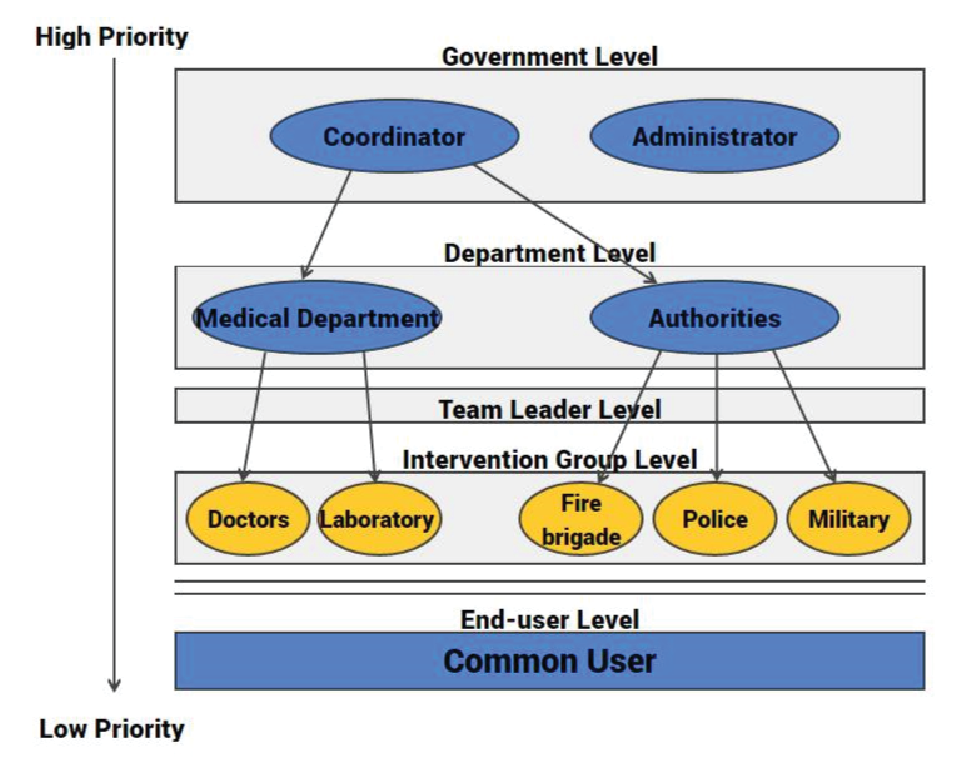
\includegraphics{images/ActorLevels.eps} \\

\subsubsection{CrisYs Corp}
CrisYs Corp are the developers of the crisis management system SHeavy.\\
\begin{description}
 \item[$\bullet$] Create and set up the system.
\end{description} 

\subsubsection{Common Users}
A common user is defined as an end user who uses SHeavy only in order to
collect information about the possible epidemic and uses the given instructions
to avoid the infection.\\
\begin{description}
 \item[$\bullet$] Common users are the principle target of SHeavy. They are
 going to use the application in order to reach information about a possible
 or several epidemic and follow the instructions given by SHeavy. 
 \item[$\bullet$]Common users will get warnings if accessing an infected
zone by GPS tracking. They will have paths to follow to access and find the
safe zones.
\end{description}

\subsubsection{Coordinators}
The Coordinator is the intermediate between its two low-level departements,
Medical Departement and Authorities, and the Government. He will execute the
orders of the Government by using SHeavy. The Coordinator has several main
functions such as :
\begin{description}
 \item[$\bullet$] The Coordinator starts or beends the alert of the concerning
 epidemic.
 \item[$\bullet$] He's also responsable for the Ressources Management, which is
 already set up before the epidemic.
 \item[$\bullet$] Another task is to update SHeavy's Map accordingly to the
 situation.
\end{description} 

\subsubsection{Administrator}
The Administrator is the responsable who keeps the ssystem operational.
Additionly he distributs the logins and the professional web and mobile
interface.
\begin{description}
 \item[$\bullet$] The Administrator keeps the system operational by maintaining
 the system.
 \item[$\bullet$] If necessary he performs some improvements and bugs
 corrections.
 \item[$\bullet$] The Administrator distributs the professional web and mobile
 interface to the concerned persons. and also the logins.
 \item[$\bullet$]  The admistrator is able to block a mobile phone or desktop
 interface for the security of the system.
\end{description} 

\subsubsection{Medical Departement}
The Medical Departement has two main groups, namely Doctors and the Laboratory.
Each one is connected with each other and they are exchanging their reports. The
Medical Departement is the intermediate between its groups and the Coordinator.
\begin{description}
 \item[$\bullet$] Sends an alert of a possible epidemic to the Coordinator.
 \item[$\bullet$] Sends several reports to the Coordinator.
\end{description} 

\subsubsection{Doctors}
Doctors are in charge of taking care of the infected victims. They'll also
perform check ups and send reports and blood sample to the Laboratory.
\begin{description}
 \item[$\bullet$] Write reports that will be sent to the Laboratory and Medical
 Departement.
 \item[$\bullet$] Works in various check points or hospitals in order to perfom
 check ups.
 \item[$\bullet$] Take care of the infected patients the time that an antivirus
 is found.
 \item[$\bullet$] Takes blood sample from the infected patients and sends them
 to the Laboratory.
\end{description} 

\subsubsection{Laboratory}
The Laboratory is a medical group which goal is to find a cure against the
virus. In constant collaboration with different medical chiefs they will get
relevant information of the evolution of the epidemic in realtime. They also get the
blood samples and reports from the Doctors.
\begin{description}
 \item[$\bullet$] Write reports that will be sent to the Doctors and Medical
 Departement.
 \item[$\bullet$] Analizing the blood samples to isolate the virus and demantle
 its structure to provide an antivirus.
 \item[$\bullet$] Gives a guideline to the application as a news so that all the
 people knows how to protect itself from become infected.
\end{description} 

\subsubsection{Authorities}
The Authorities is regrouping various intervention groups such as the fire
brigade, the police and the militaries. They are working together and have a
connection with each other. The Authorities are the intermediate between its
groups and the Coordinator.
\begin{description}
 \item[$\bullet$] Support group for various purposes. 
\end{description}

\subsubsection{Team Leader}
Team Leader are present in all instances of epartements such as Medical
Departements and Authorities. They are the leader of an intervention group which
is going to execute missions given by the Coordinator.
\begin{description}
 \item[$\bullet$] They are responsable of his team.
 \item[$\bullet$] Accept or decline a mission given by the Coordinator.
 \item[$\bullet$] Execute missions.
\end{description}

\subsection{Operating environment}
SHEAVY is a webbased application. It has a server and a client side. The server
needs to be powerfull to handle the mass of information. Clients need to have a
good internet access and a basic system requirement to access fast their
pages.\\

\subsubsection{System requirements: Client}
\begin{tabular}{|c|c|}
\hline
\multicolumn{2}{|c|}{\textbf{Phone Application}} \\
\hline
\multicolumn{2}{|c|}{\textit{\textbf{Android}}} \\
\hline
OS & Android \\
\hline
Hardware & ARM 5 Dual Core \\
\hline
\multicolumn{2}{|c|}{\textit{\textbf{iOS}}} \\
\hline
Operating System & iOS 8 \\
\hline
Hardware & iPhone 5 \\
\hline
\end{tabular}

\subsubsection{System requirements: Server}
\begin{tabular}{|c|c|}
\hline
\multicolumn{2}{|c|}{\textbf{Server Application}} \\
\hline
\multicolumn{2}{|c|}{\textit{\textbf{Linux x86/x64}}} \\
\hline
Kernel & 4.8.1 \\
\hline
Hard disk space & 10 TB   \\
\hline
Processeur & Intel Xeon E7-8893 \\
\hline
RAM & 32 GB \\
\hline
\end{tabular}

\section{Document structure}  
Information on how this document is organised and it is expected to be
used. Recommendations on which members of the audience
should consult which sections of the document, and explanations about the used
notation (i.e. description of formats and conventions) must also be provided.\\









\newpage

% User guide
\chapter{Usage Guide}
\label{chap:usage_guide}

This section is aimed at describing the general use of the software. Such
information is grouped by the different kinds of actors.
Such actors are expected to use the software to perform some
processes or workflows (called here procedures) using the concerned software
\textbf{(including installation procedures)}.

\section{Actors common procedures}
Common procedures to several actors are grouped in this section to avoid
redundancy.

\subsection{Application Installation}
\vspace{0.5cm}
\hrule
\vspace{0.5cm}
\begin{lyxlist}{UC1}
\small{
\item [\textbf{Use~Case:}] ApplicationInstallation
\item [\textbf{Scope:}] Crisis Management System \textbf{(\emph{SHeavy})}
\item [\textbf{Primary Actor}:] Every user
\item [\textbf{Secondary Actor}:] None
\item [\textbf{Intention:}] Every single user who is going to use SHeavy on
their mobile have to proceed the installation.
\item [\textbf{Level}:]Sub-functional level
\item [\textbf{Main~Success~Scenario}]:\\
1. The user has to open their respective mobile store applicaton.\\
2. He has to search for SHeavy in the searchbar.\\
3. Then he as to confirm the installation by accepting the terms.\\
4. The application was installed succesfully and the user can start using the
application.\\
Extensions:\\
1.a If the user uses an iOS device, he has to open the apple store.\\
1.b If the user uses an android device, he has to open the play store.\\	
}
\end{lyxlist}
\hrule 
\vspace{0.5cm}

\subsection{Find a Person}
\vspace{0.5cm}
\hrule
\vspace{0.5cm}
\begin{lyxlist}{UC1}
\small{
\item [\textbf{Use~Case:}] FindPerson
\item [\textbf{Scope:}] Crisis Management System \textbf{(\emph{SHeavy})}
\item [\textbf{Primary Actor}:] Medical Departement, Government
\item [\textbf{Secondary Actor}:] Medical Departement, Government
\item [\textbf{Intention:}]A user except to common users can find people by name, by availablity or by
his functionality and call them.
\item [\textbf{Level}:]Subfunctional level
\item [\textbf{Main~Success~Scenario}]:\\
1. A User access the contact Menu.\\
2. A User input the name, fonctionality and get a list of matches.\\
3. A User can call or write a message to the specific user.\\
Extensions:\\ 
	1.a. A common user get just access to the Call Centers lines.\\
}
\end{lyxlist}
\hrule 
\vspace{0.5cm} 

\subsection{Finding safe route}
\vspace{0.5cm}
\hrule
\vspace{0.5cm}
\begin{lyxlist}{UC1}
\small{
\item [\textbf{Use~Case:}] FindSafe
\item [\textbf{Scope:}] Crisis Management System \textbf{(\emph{SHeavy})}
\item [\textbf{Primary Actor}:] System
\item [\textbf{Secondary Actor}:] Every User
\item [\textbf{Intention:}]Suggest the user the safest way to get to a safe
place (e.g. hospital).
\item [\textbf{Level}:]Sub-functional level
\item [\textbf{Main~Success~Scenario}]:\\
1. The user access the SafePlaceFinder in the menu bar of the application.\\
2. The user select a place to go.\\
3. The user's GPS application opens with the route.\\
Extensions:\\
3.a SHeavy calculates the fastest way avoiding Unsafe and Danger Zones.\\
	3.a.1 SHeavy ignores any way through an Unsafe/Danger Zone.\\
	3.a.2 SHeavy calculates the fastest way from the non-ignored ways.\\
\item 
}
\end{lyxlist}
\hrule
\vspace{0.5cm}

\subsection{Accept Mission}
\vspace{0.5cm}
\hrule
\vspace{0.5cm}
\begin{lyxlist}{UC1}
\small{
\item [\textbf{Use~Case:}] AcceptMission
\item [\textbf{Scope:}] Crisis Management System \textbf{(\emph{SHeavy})}
\item [\textbf{Primary Actor}:] Medical Departement, Authorities
\item [\textbf{Secondary Actor}:] Coordinator
\item [\textbf{Intention:}]The Teamleader accepts a mission.
\item [\textbf{Level}:]Sub-functional level
\item [\textbf{Main~Success~Scenario}]:\\
1. The Teamleader gets a notification on his mobile application.\\
2. The Teamleader accept or decline the mission.\\
Extensions:\\
	2.a. If accepted the mission will be sent to his team members.\\
	2.b. If declined the mission will be affected to another team.\\ 
}
\end{lyxlist}
\hrule 
\vspace{0.5cm} 

\section{Administrator procedures}

\subsection{Software Installation}
\vspace{0.5cm}
\hrule
\vspace{0.5cm}
\begin{lyxlist}{UC1}
\small{
\item [\textbf{Use~Case:}] SoftwareInstallation
\item [\textbf{Scope:}] Crisis Management System \textbf{(\emph{SHeavy})}
\item [\textbf{Primary Actor}:] Adminstrator
\item [\textbf{Secondary Actor}:] Coordinator, Medical Departement, Authorities
\item [\textbf{Intention:}] The Adminstrator will install for the concerned,
namely  Coordinator, Medical Departement, Authorities, actors a software in
their desktop.
\item [\textbf{Level}:]Sub-functional level
\item [\textbf{Main~Success~Scenario}]:\\
1. The Adminstrator starts the installation in the specifs desktops.\\
2. He will also configure the settings.\\
3. He'll also perfom a test run.\\
4. The software is successfully installed.\\
Extensions:\\
2.a The test run fails and the adminstrator will repair it.\\
}
\end{lyxlist}
\hrule 
\vspace{0.5cm}

\section{Coordinator procedures}

\subsection{Trigger The Alert State}
\vspace{0.5cm}
\hrule
\vspace{0.5cm}
\begin{lyxlist}{UC1}
\small{
\item [\textbf{Use~Case:}] TriggerAlertState
\item [\textbf{Scope:}] Crisis Management System \textbf{(\emph{SHeavy})}
\item [\textbf{Primary Actor}:] Coordinator
\item [\textbf{Secondary Actor}:] Medical Departement
\item [\textbf{Intention:}] According to the diagnostic made by the Medical
Departement, which will be sent to the Coordinator, the Coordinator will trigger
the alert and SHeavy will notify all users about a possible epidemic.
\item [\textbf{Level}:]Sub-functional level
\item [\textbf{Main~Success~Scenario}]:\\
1. The Doctor notice that a patient is contracting an highly infectious virus.\\
2. The Doctor sends the report and blood samples to the Laboratory.\\
3. The Laboratory proceed to various tests with the blood samples.\\
4. If the risk of a possible epidemic is assesssed, a report wil be sent to
the Coordinator.\\
5. The Coordinstor recieves the report and trigger the alert of an epidemic.\\
Extensions:\\
4.a The tests shows their's no risk of epidemic and no report will be sent to
the Coordinator.\\
}
\end{lyxlist}
\hrule 
\vspace{0.5cm} 

\subsection{Lift The Alert Atate}
\vspace{0.5cm}
\hrule
\vspace{0.5cm}
\begin{lyxlist}{UC1}
\small{
\item [\textbf{Use~Case:}] LiftAlertState
\item [\textbf{Scope:}] Crisis Management System \textbf{(\emph{SHeavy})}
\item [\textbf{Primary Actor}:] Coordinator
\item [\textbf{Secondary Actor}:] Medical Departement
\item [\textbf{Intention:}] According to the diagnostic made by the Medical
Departement,which is send to the Coordinator, the Coordinator
will lift of the epidemic and SHeavy will notify all users that the epidemic is
over.
\item [\textbf{Level}:]Sub-functional level
\item [\textbf{Main~Success~Scenario}]:\\
1. The Laboratory finds a cure for the epidemic.\\
2. All infected persons are healed.\\
3. The Medical Departement sends a report to the Coordinator, in which it is
said that the epidemic is over.\\
4. The Coordinator reads the report and according to that lift the alert.\\ 
}
\end{lyxlist}
\hrule
\vspace{0.5cm} 

\subsection{Handling Ressources}
\vspace{0.5cm}
\hrule
\vspace{0.5cm}
\begin{lyxlist}{UC1}
\small{
\item [\textbf{Use~Case:}] OverView
\item [\textbf{Scope:}] Crisis Management System \textbf{(\emph{SHeavy})}
\item [\textbf{Primary Actor}:] Coordinator
\item [\textbf{Secondary Actor}:] Medical Departement, Authorities
\item [\textbf{Intention:}] The Coordinator gets an overview of the infected
zone, it's infrastructures and the deployed teams.
\item [\textbf{Level}:]Sub-functional level
\item [\textbf{Main~Success~Scenario}]:\\
1. The Coordinator access his webinterface.\\
2. The Coordinator clicks on OVERVIEW in the menu.\\
Extensions:\\
	2.a. He can filter the information.\\
}
\end{lyxlist}
\hrule
\vspace{0.5cm} 

\subsection{Send Mission}
\vspace{0.5cm}
\hrule
\vspace{0.5cm}
\begin{lyxlist}{UC1}
\small{
\item [\textbf{Use~Case:}] SendMission
\item [\textbf{Scope:}] Crisis Management System \textbf{(\emph{SHeavy})}
\item [\textbf{Primary Actor}:] Coordinator
\item [\textbf{Secondary Actor}:] Medical Departement, Authorities
\item [\textbf{Intention:}]The Coordinator sent a mission to a teamleader.
\item [\textbf{Level}:]Sub-functional level
\item [\textbf{Main~Success~Scenario}]:\\
1. The Coordinator access the MISSION menu in his webinterface.\\
2. The Coordinator choose Submit Mission.\\
3. The Coordinator fulfill the information.\\
4. The Coordinator sends the notification.\\
}
\end{lyxlist}
\hrule 
\vspace{0.5cm} 

\subsection{Set Zone}
\vspace{0.5cm}
\hrule
\vspace{0.5cm}
\begin{lyxlist}{UC1}
\small{
\item [\textbf{Use~Case:}] SetZone
\item [\textbf{Scope:}] Crisis Management System \textbf{(\emph{SHeavy})}
\item [\textbf{Primary Actor}:] Coordinator
\item [\textbf{Secondary Actor}:] Laboratory
\item [\textbf{Intention:}] Set up a safe camp or a quarantine zone.
\item [\textbf{Level}:]Sub-functional level
\item [\textbf{Main~Success~Scenario}]:\\
1. The Laboratory surveys the status of a zone.\\
2. After the Laboratory confirms that a zone is safe or infected, the
Coordinator is notified.\\
3. The Coordinator will set a new camp and Sheavy will notify all the users
automatically.\\ 
4.	The Coordinator will sent a request to the concerned intervention groups to
set the camp.\\
}
\end{lyxlist}
\hrule
\vspace{0.5cm} 

\subsection{Change Zone State}
\vspace{0.5cm}
\hrule
\vspace{0.5cm}
\begin{lyxlist}{UC1}
\small{
\item [\textbf{Use~Case:}] ChangeZoneState
\item [\textbf{Scope:}] Crisis Management System \textbf{(\emph{SHeavy})}
\item [\textbf{Primary Actor}:] Coordinator
\item [\textbf{Secondary Actor}:] Laboratory
\item [\textbf{Intention:}] Change the state of an already set zone.
\item [\textbf{Level}:]Sub-functional level
\item [\textbf{Main~Success~Scenario}]:\\
1. The Laboratory surveys the status of a zone.\\
2. The Laboratory send futher reports to the Coordinator about the change of a
zone.\\
3. The Coordinator reads the reports and change the zone state and SHeavy will
notify all the users.\\
}
\end{lyxlist}
\hrule
\vspace{0.5cm} 

\section{Doctor procedures}

\subsection{Handling of infected patient}
\vspace{0.5cm}
\hrule
\vspace{0.5cm}
\begin{lyxlist}{UC1}
\small{
\item [\textbf{Use~Case:}] HandlingOfInfectedPatient
\item [\textbf{Scope:}] Crisis Management System \textbf{(\emph{SHeavy})}
\item [\textbf{Primary Actor}:] Doctor
\item [\textbf{Secondary Actor}:] Labotatory
\item [\textbf{Intention:}]The Medical Department intends to update
the application with the newest data about infected people, no matter what
sickness they have. In case of a known epidemic infection, keep an updated
record of the growth of the epidemic.
\item [\textbf{Level}:]Sub-functional level
\item [\textbf{Main~Success~Scenario}]:\\
1. The Doctor performs a medical check on a patient.\\
2. He writes or updates data about the patient in his report.\\
3. The Doctor sends the blood sample to the nearest laboratory in order to find
a cure.\\
4. The Doctor tries to stop the infection by performing several operations or
by followinf the instruction of the Laboratory.\\
}
\end{lyxlist}
\hrule
\vspace{0.5cm} 

\section{Common Users Procedures}

\subsection{Alert While Entering a Danger Zone}
\vspace{0.5cm}
\hrule
\vspace{0.5cm}
\begin{lyxlist}{UC1}
\small{
\item [\textbf{Use~Case:}] DangerAlert
\item [\textbf{Scope:}] Crisis Management System \textbf{(\emph{SHeavy})}
\item [\textbf{Primary Actor}:] Common user
\item [\textbf{Secondary Actor}:] None
\item [\textbf{Intention:}]Warn a user that he is about to enter a Danger Zone 
before entering the Danger Zone.
\item [\textbf{Level}:]Sub-functional level
\item [\textbf{Main~Success~Scenario}]:\\
1. The common user is going somewhere in or near a Danger Zone to do
something.\\
2. The common user is located by SHeavy and John is near a Danger Zone and is
going in its direction.\\
3. SHeavy immediately send a warning to John's Phone, indicating 
that John is entering a Danger Zone.\\
4. The common user sees the warning and he takes a way around the Danger Zone.\\
}
\end{lyxlist}
\hrule
\vspace{0.5cm} 




















\newpage

% Software operations
\chapter{Software operations}
\label{chap:soptware_operations}


Explain each allowed software operations (i.e. an atomic unit of treatment, a service, a functionality) including a brief description of the operation, required parameters, optional parameters, default options, required steps to trigger the operation, assumptions upon request of the operation and expected results of executing such operation.
Describe how to recognise that the operation has successfully been executed or
abnormally terminated. The template given below (i.e. section \ref{operation:MyOperation} has to be used).

Group the operations devoted to the needs of specific actors. Common
operations to several actors may be grouped and presented once to avoid redundancy.


\section{MyOperation}
\label{operation:MyOperation}
The system operator creates and adds a new crisis to the system after being
informed by a third party (citizen, organization) and selects a crisis handler for the crisis.
 
\subsection{MyExample1}
Examples should illustrate the use of \textbf{complex operations}.

Each example must show how the actor uses the software operation under
description to achieve (at least one of) its expected outcome.

It might be required to include GUI screenshots to illustrate the example.\\

\section{Login}
\label{operation:Login}
The coordinator, administrator, leaders or anyone working in the medical
department or authorities wants to access the applications.\\
\begin{description}
\item \textbf{Parameters:} User Information, User Password
\item \textbf{Precondition:} The user has the application open.
\item \textbf{Post-condition:}  The user enters the homescreen with access to
his individual information and functions.
\item \textbf{Output messages:} None.
\item \textbf{Triggering:}
\begin{enumerate}
\item After opening the application the user has two textfields for accound and
password.
\item The user enters his accound and his password.
\item Click on the 'Login' button and the user will be linked to the homescreen.
\end{enumerate}
\end{description}


\section{Send Alert}
\label{operation:SendAlert}
The Medical Departement creates an alert message for an epidemic, including a
report of what happened and what should be done as a reaction of that epidemic.
He's sending it to the Coordinator who will read it and confirm the alert
state.\\
\begin{description}
\item \textbf{Parameters:} Alert Information, User and State Information
\item \textbf{Precondition:} The user is logged in as professional user such as
Medical Departement.
\item \textbf{Post-condition:}  The alert was successfully sent and the
Coordinator was notified about the alert.
\item \textbf{Output messages:} 'Alert sent'.
\item \textbf{Triggering:}
\begin{enumerate}
\item In the alert message window, the professional user fills out the alert
information: the title and the description text-fields.
\item The message has to have an report as well as indicating the state of the
alert if needed.
\item Click on the 'Send' button and the Coordinator will be notified of the
epidemic.
\end{enumerate}
\end{description}

\section{Confirm Alert}
\label{operation:ConfirmAlert}
The Coordinator recieves an alert message from the Medical Departement
including a report about the severity of the epidemic. The Coordinator will
read it and will confirm the alert and notify every user about the epidemic.\\
\begin{description}
\item \textbf{Parameters:} Alert Information, User and State Information
\item \textbf{Precondition:} The user is logged in as professional user and
has already read the report.
\item \textbf{Post-condition:} Start of the CMS. The alert is confirmed and
every user is notified about he epidemic.
\item \textbf{Output messages:} 'Epidemic confirmed'.
\item \textbf{Triggering:}
\begin{enumerate}
\item The Coordinator recieves an alert notification on his web-interface. He
has to click on 'Report' to read the report sent by the Medical Departement.
\item According to the Coordinator's decision he'll click on 'Launch Crisis' to
start the crisis, 'Delay Decision' to not decide yet if he needs confirmation of
the governement or 'Decline' if the situaton don't need a crisis
management system.
\end{enumerate}
\end{description}

\section{Upgrade User to Professional status}
\label{operation:UpgradeUser}
In request of the coordinator, the Administrator wants to upgrade a common user
to a professional user.\\
\begin{description}
\item \textbf{Parameters:} User name, Coordinator Request
\item \textbf{Precondition:} The administrator has to be on his home screen.
\item \textbf{Post-condition:}  The selected user gains access to the new
feature of the system.
\item \textbf{Output messages:} None.
\item \textbf{Triggering:}
\begin{enumerate}
\item The administrator selects or he uses the search to find and select the
requested user in order to modify his data.
\item The administrator selects the requested type of professonal from the
following: Common User, Medical Department, Authorities and Coordinator.
\item The administrator selects his subtype for the Medical Department and
Authorities but not for the Common user and Coordinator.
\item The system modify the information as the administrator changes the
selectboxes.
\end{enumerate}
\end{description}

\section{Find Safe Place}
\label{operation:FindSafePlace}
Any user requests the safest and fastest way to a certain safe place e.g. hospital,
safe camp. The operation will send him through GPS to the selected place.\\
\begin{description}
\item \textbf{Parameters:} Place Information, Place Location
\item \textbf{Precondition:} The user is logged in and has his GPS enabled.
\item \textbf{Post-condition:}  The fastest way to a certain safe place was
calculated.
\item \textbf{Output messages:} 'Route to the selected safe place is ready.'
\item \textbf{Triggering:}
\begin{enumerate}
\item In the menu the user clicks on 'Safe Place Finder'.
\item A new window shows a list of safe places and the user choses one by 
clicking on the one the user wants to request the route and send the Place Information to SHeavy.
\item SHeavy send back the Place Location which includes the actual location as well as the safest route.
\item The user is lead to the GPS window.
\end{enumerate}
\end{description}

\section{Urgency Call}
\label{operation:UrgencyCall}
Any professional user requests a call to a specific group in a certain location by selecting 
them in the contact list or using the search to find the group (medics, fireman, military) 
by name or location (e.g. hospital/camp name or city they are located).\\
\begin{description}
\item \textbf{Parameters:} Contact Information
\item \textbf{Precondition:} The user is logged in and has to be connected to a
nnetwork.
\item \textbf{Post-condition:} The application uses call the respective group or person.
\item \textbf{Output messages:} Calling 'ContactX'
\item \textbf{Triggering:}
\begin{enumerate}
\item Open the 'Contacts'-menu.
\item Searchs for the person to call.
\item Click on 'Call' to request a call to the person or group.
\end{enumerate}
\end{description} 

\section{Set Camp Mission}
\label{operation:SetCampMission}
The Coordinator sends set camp mission to various groups leaders (e.g. fire
figther, military, Doctors,..) with some important information concerning the
mission.\\
\begin{description}
\item \textbf{Parameters:} Contact Information, Mission Information
\item \textbf{Precondition:} The user is logged in as a professional user.
\item \textbf{Post-condition:} The mission is recieved by the concerned leader.
\item \textbf{Output messages:} 'Mission Pending'
\item \textbf{Triggering:}
\begin{enumerate}
\item The Coordinator opens the 'Mission-view'.
\item Select one or more teams by selecting a leader in the 'send to' field or
sends to all by clicking on 'Send to All'.
\item Writes the title and select 'Set Camp' as type by clicking on 'Set
Type'.
\item Give the Location of the camp and also announce a deadline in format Date
and time.
\item Furthermore indicates de capacity of the camp and how many teams are
needed there.
\item Fill the description for more details about the mission.
\item Click on the 'Send'-Button to submit the mission.
\end{enumerate}
\end{description}

\section{Set Checkpoint Mission}
\label{operation:CheckpointMission}
The Coordinator sends set checkpoint mission to various groups leaders (e.g.
fire figther, military, Doctors,..) with some important information concerning the
mission.\\
\begin{description}
\item \textbf{Parameters:} Contact Information, Mission Information
\item \textbf{Precondition:} The user is logged in as a professional user.
\item \textbf{Post-condition:} The mission is recieved by the concerned leader.
\item \textbf{Output messages:} 'Mission Pending'
\item \textbf{Triggering:}
\begin{enumerate}
\item The Coordinator opens the 'Mission-view'.
\item Select one or more teams by selecting a leader in the 'send to' field or
sends to all by clicking on 'Send to All'.
\item Writes the title and select 'Set Checkpoint' as type by clicking on 'Set
Type'.
\item Give the Location of the camp and also announce a deadline in format Date
and time.
\item Furthermore indicates how many teams are needed there and where victims
are going to be moved.
\item Fill the description for more details about the mission.
\item Click on the 'Send'-Button to submit the mission.
\end{enumerate}
\end{description} 

\section{Transfer Mission}
\label{operation:TransferMission}
The Coordinator sends transfer mission to various groups leaders (e.g. fire
figther, military, Doctors,..) with some important information concerning the
mission.\\
\begin{description}
\item \textbf{Parameters:} Contact Information, Mission Information
\item \textbf{Precondition:} The user is logged in as a professional user.
\item \textbf{Post-condition:} The mission is recieved by the concerned leader.
\item \textbf{Output messages:} 'Mission Pending'
\item \textbf{Triggering:}
\begin{enumerate}
\item The Coordinator opens the 'Mission-view'.
\item Select one or more teams by selecting a leader in the 'send to' field or
sends to all by clicking on 'Send to All'.
\item Writes the title and select 'Transfer People' as type by clicking on 'Set
Type'.
\item Give the Locations from where to where people are going to be moved.
\item Announce a deadline in format Date and time and how many people are going
to be moved.
\item Click on the 'Send'-Button to submit the mission.
\end{enumerate}
\end{description}

\section{Evacuation Mission}
\label{operation:EvacuateMission}
The Coordinator sends evacuation mission to various groups leaders (e.g. fire
figther, military, Doctors,..) with some important information concerning the
mission.\\
\begin{description}
\item \textbf{Parameters:} Contact Information, Mission Information
\item \textbf{Precondition:} The user is logged in as a professional user.
\item \textbf{Post-condition:} The mission is recieved by the concerned leader.
\item \textbf{Output messages:} 'Mission Pending'
\item \textbf{Triggering:}
\begin{enumerate}
\item The Coordinator opens the 'Mission-view'.
\item Select one or more teams by selecting a leader in the 'send to' field or
sends to all by clicking on 'Send to All'.
\item Writes the title and select 'Evacuate' as type by clicking on 'Set
Type'.
\item Give the Locations from where to where people are going to be evacuate.
\item Indicate an estimated number of people to be rescued but can be changed
lately.
\item Click on the 'Send'-Button to submit the mission.
\end{enumerate}
\end{description}

\section{Accept Mission}
\label{operation:AcceptMission}
Each group member can recieve a mission from the Coordinator. But only the
leader can accept the mission or decline if they can't execute it.\\
\begin{description}
\item \textbf{Parameters:} Contact Information, Mission Information
\item \textbf{Precondition:} The user is logged in as a professional user
and recieves the mission notification.
\item \textbf{Post-condition:} The mission will be executed or sent to another
team.
\item \textbf{Output messages:} The mission is Accepted or Transfer.
\item \textbf{Triggering:}
\begin{enumerate}
\item The team leader recieves a mission.
\item He can click on 'Details' to get further information or decline
immimediately.
\item By clickin ont 'Extras' he get information about other teams present in
the mission zone.
\item He can click on 'Accept' or 'Decline'
\item After accepting the mission he gets a confirmation notification. He can
quit it by clicking on 'OK'.
\end{enumerate}
\end{description} 

\section{Add New Zone}
\label{operation:AddNewZoneS}
The Coordinator can add new zones to the map. According to that the map will
be updated.\\
\begin{description}
\item \textbf{Parameters:} Epidemic Information, Change State
\item \textbf{Precondition:} The user is logged in as a professional user.
\item \textbf{Post-condition:} A new zone was added to the map.
\item \textbf{Output messages:} 'Updated'
\item \textbf{Triggering:}
\begin{enumerate}
\item The Coordinator opens the 'Map Editor-view'.
\item He has to click on the 'Add Zone' label to add a new Zone.
\item He has to select a Type of zone by clicking on 'Choose Type'.
\item The Coordinator select the visibility type.
\item Set the area by given an estimation of the height and width in km.
\item At last select the Location where the area will be set.
\item Click on the 'Add Zone'-Button to submit the modifications
on the map.
\end{enumerate}
\end{description} 

\section{Change Zone}
\label{operation:ChangeZone}
The Coordinator can change a zone's propreties in any time. According
to that the map will be updated.\\
\begin{description}
\item \textbf{Parameters:} Epidemic Information, Change State
\item \textbf{Precondition:} The user is logged in as a professional user.
\item \textbf{Post-condition:} An existing zone was modified on the map.
\item \textbf{Output messages:} 'Updated'
\item \textbf{Triggering:}
\begin{enumerate}
\item The Coordinator opens the 'Map Editor-view'.
\item He has to click on the 'Set Zone' label to change a Zone.
\item At first he has to select the zone by clicking on 'Select a Zone' button
or searches for the name of the zone.
\item He can modify the zone's propreties.
\item Click on the 'Safe Changes' to submit the modifications
on the map or click on 'Cancel Changes' to cancel the modification.
\end{enumerate}
\end{description} 

\section{Delete Zone}
\label{operation:DeleteZone}
The Coordinator can delete a zone in any time. According
to that the map will be updated.\\
\begin{description}
\item \textbf{Parameters:} Epidemic Information, Change State
\item \textbf{Precondition:} The user is logged in as a professional user.
\item \textbf{Post-condition:} An existing zone was deleted on the map.
\item \textbf{Output messages:} 'Updated'
\item \textbf{Triggering:}
\begin{enumerate}
\item The Coordinator opens the 'Map Editor-view'.
\item He has to click on the 'Set Zone' label to change a zone.
\item At first he has to select the zone by clicking on 'Select a Zone' button
or searches for the name of the zone.
\item Click on the 'Delete Zone' button to delete the zone or click on the
'Cancel Change' button to quit.
\end{enumerate}
\end{description} 

\section{Requirements}
\label{operation:Requirements}
The professional user (medical department, authorities) can
request material needs or support by a resource team. The user has to describe
the needs in the corresponding window.\\
\begin{description}
\item \textbf{Parameters:} Needs Information, Needs Request
\item \textbf{Precondition:} The user has to be logged in as professional.
\item \textbf{Post-condition:}  The request is send to the corresponding groups.
\item \textbf{Output messages:} None
\item \textbf{Triggering:}
\begin{enumerate}
\item Click on menu, then resource and then on needs.
\item The user has to fill out the Needs Information that is the selection of
the receiver, as well as the description of the needs.
\item The user has to indicate his location to add a verification of the needs. 
\item After filling in, click on 'Send' to notify the resource teams of your
request.
\item The user will be notify after the receiver confirms the request. 
\end{enumerate}
\end{description}




\newpage

% Error messages and problem resolution

\chapter{Error messages and problem resolutions}
\label{chap:error_messages}

All known problems in using the software should be listed and explained in
details using the structure presented below.

Contact information for reporting any problems (either with the software or
this document) should be clearly indicated


\section{No Mobile Network}

\subsection{Problem identification}
Impossible to refresh or to get the latest news or notifications.\\
Impossible to opens some features of the application.

\subsection{Probable cause}
The user may have put the device in flight mode, has no Wifi or is out of the
router's range or no mobile connection. It may be that the main server isn't
operational any more or a misfunction from your ISP. The router can also be
turned off.

\subsection{Corrective actions}
\begin{description} 
\item[$\bullet$] The user may reduce the range between the router and the mobile
phone.
\item[$\bullet$] Contact your Internet service provider.
\item[$\bullet$] Go to the Settings menu, disable the 'Flight mode' option.
\item[$\bullet$] Go to the Settings menu, enable the 'Mobile data' option.
\item[$\bullet$] Go to the Settings menu, enable the 'Wifi' option.
\item[$\bullet$] Wait until the main server is operational again.
\end{description} 

\section{No Internet Network}

\subsection{Problem identification}
Impossible to refresh or to get the latest news or notifications.\\
Impossible to opens some features of the application nor send information.

\subsection{Probable cause}
The user may have put the device in flight mode, has no Wifi or is out of the
router's range or no ethernet connection. It may be that the main server isn't
operational any more or a misfunction from your ISP. The router can also be
turned off.

\subsection{Corrective actions}
\begin{description} 
\item[$\bullet$] The user may reduce the range between the router and the
computer.
\item[$\bullet$] Turn on the router.
\item[$\bullet$] Contact your Internet service provider.
\item[$\bullet$] Go to the Settings menu, disable the 'Flight mode' option.
\item[$\bullet$] Go to the Settings menu, enable the 'Wifi' option.
\item[$\bullet$] Wait until the main server is operational again.
\end{description} 
\newpage

%APPENDICES
\appendix
\chapter{Referenced Illustrations}
\label{chap:appendix}
%Reducing the spacing from the title


\section{Screen Graphs}
\label{sec:ScreenGraph}
\subsection{Application Screens}

\subsubsection{Common User}
\center{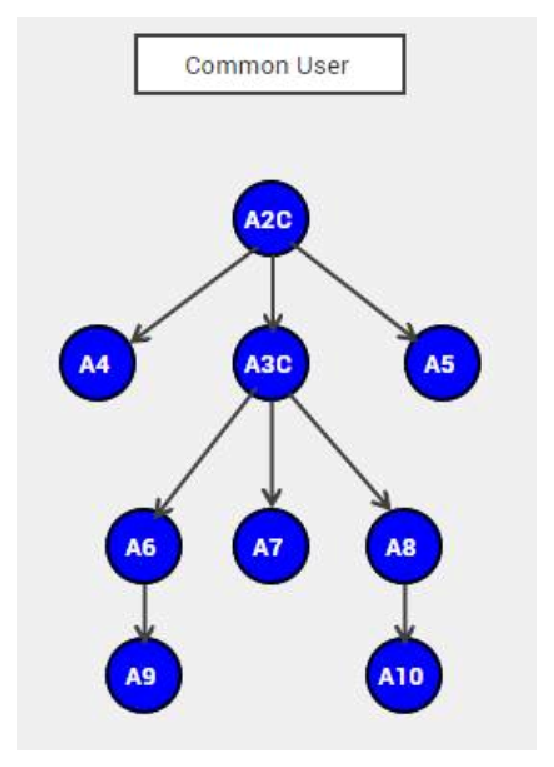
\includegraphics{images/commonuser.eps}}
\begin{figure}[htbp]
\begin{center}
 \caption{\label{fig:A2C} Home Screen}
   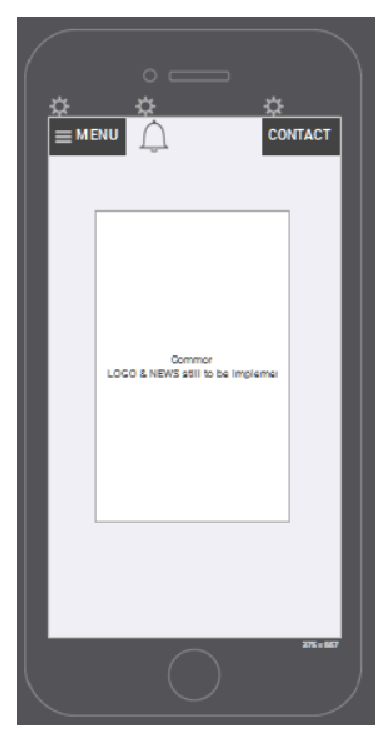
\includegraphics[width=50mm]{./images/App/chome.eps}
\end{center}
\end{figure} 
\begin{figure}[htbp]
\begin{center}
 \caption{\label{fig:A4} Alert Screen}
   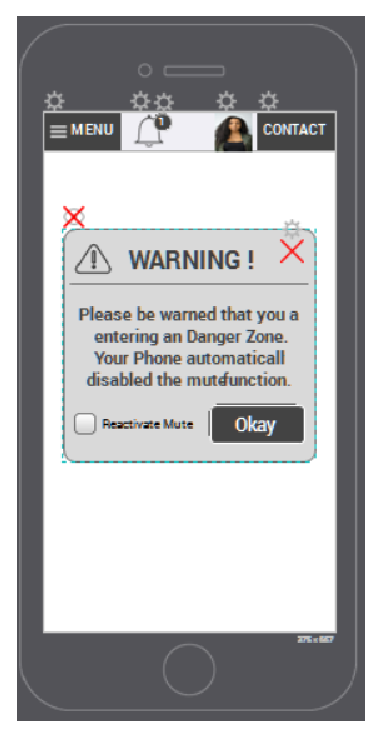
\includegraphics[width=50mm]{./images/App/alerscreen.eps}
\end{center}
\end{figure} 
\begin{figure}[htbp]
\begin{center}
 \caption{\label{fig:A5} Contact Screen}
   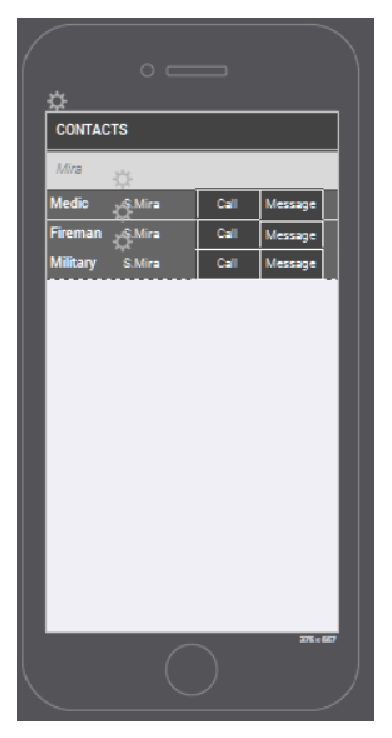
\includegraphics[width=50mm]{./images/App/contactscreen.eps}
\end{center}
\end{figure} 
\begin{figure}[htbp]
\begin{center}
 \caption{\label{fig:A3C} Menu Screen}
   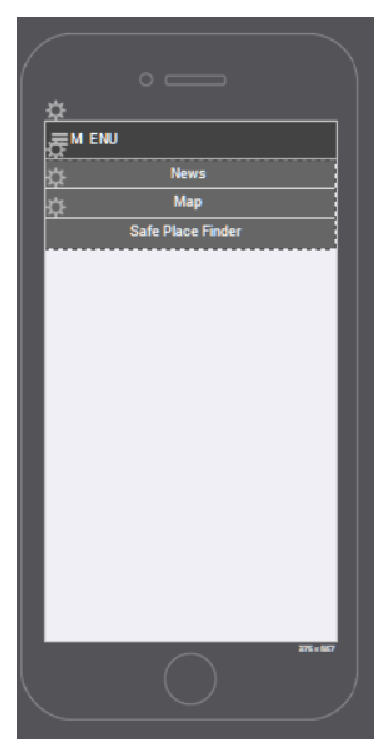
\includegraphics[width=50mm]{./images/App/cmenu.eps}
\end{center}
\end{figure} 
\begin{figure}[htbp]
\begin{center}
 \caption{\label{fig:A6} News Screen}
   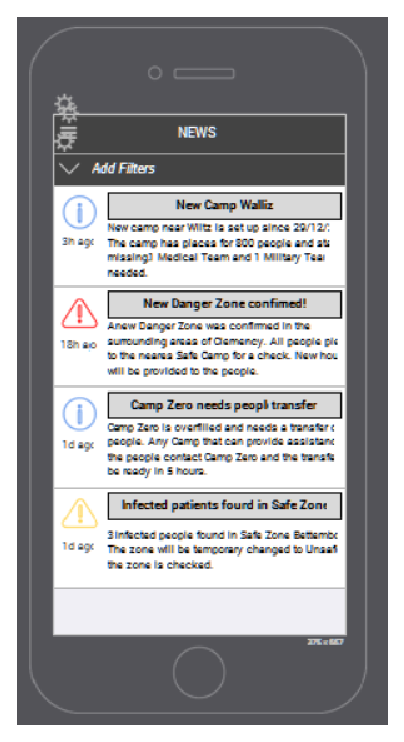
\includegraphics[width=50mm]{./images/App/newsscreen.eps}
\end{center}
\end{figure} 
\begin{figure}[htbp]
\begin{center}
 \caption{\label{fig:A7} Map Screen}
   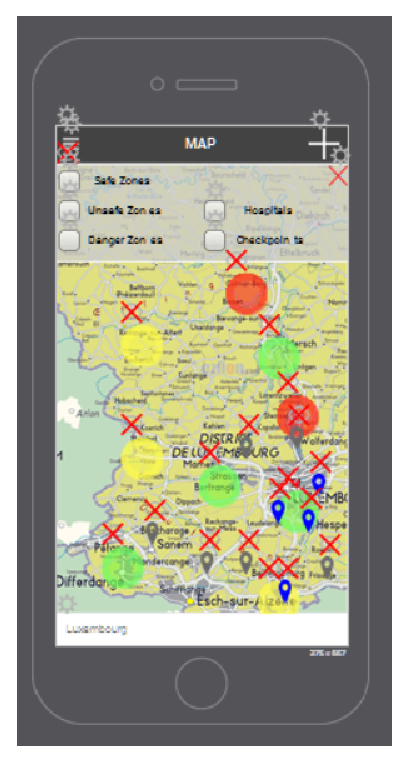
\includegraphics[width=50mm]{./images/App/mapscreen.eps}
\end{center}
\end{figure} 
\begin{figure}[htbp]
\begin{center}
 \caption{\label{fig:A8} Safe Place Finder Screen}
   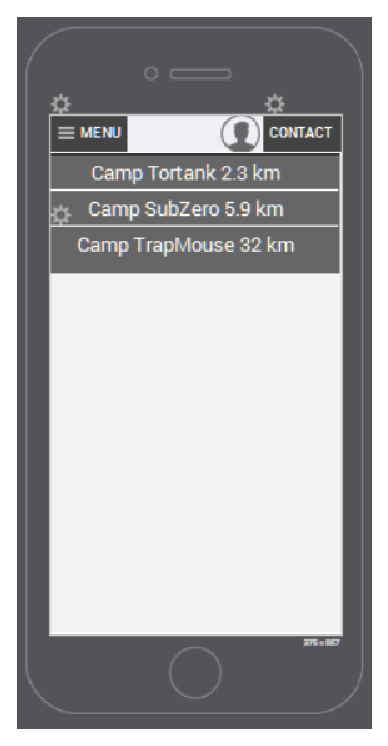
\includegraphics[width=50mm]{./images/App/placefinder.eps}
\end{center}
\end{figure} 
\begin{figure}[htbp]
\begin{center}
 \caption{\label{fig:A9}  News Filter Screen}
   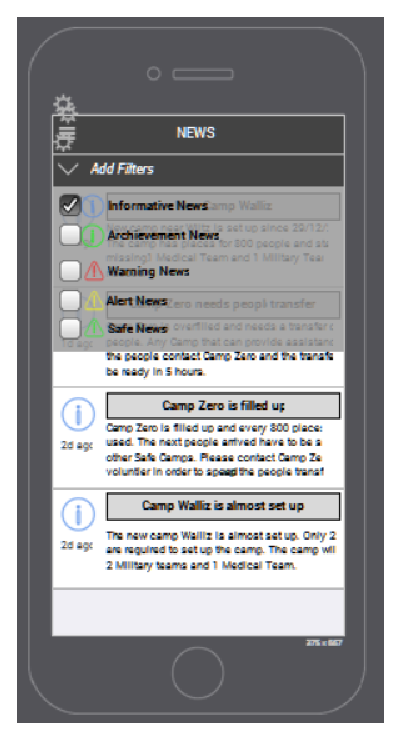
\includegraphics[width=50mm]{./images/App/newsfilter.eps}
\end{center}
\end{figure} 
\begin{figure}[htbp]
\begin{center}
 \caption{\label{fig:A10} Trace Screen}
   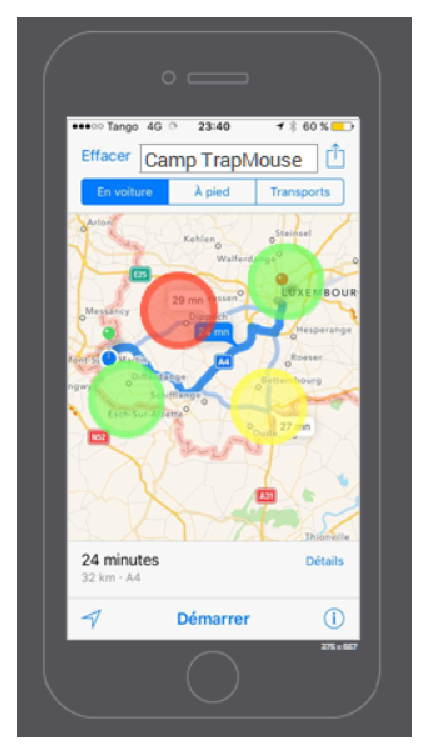
\includegraphics[width=50mm]{./images/App/traceroute.eps}
\end{center}
\end{figure} 




\subsubsection{Professional User}
\center{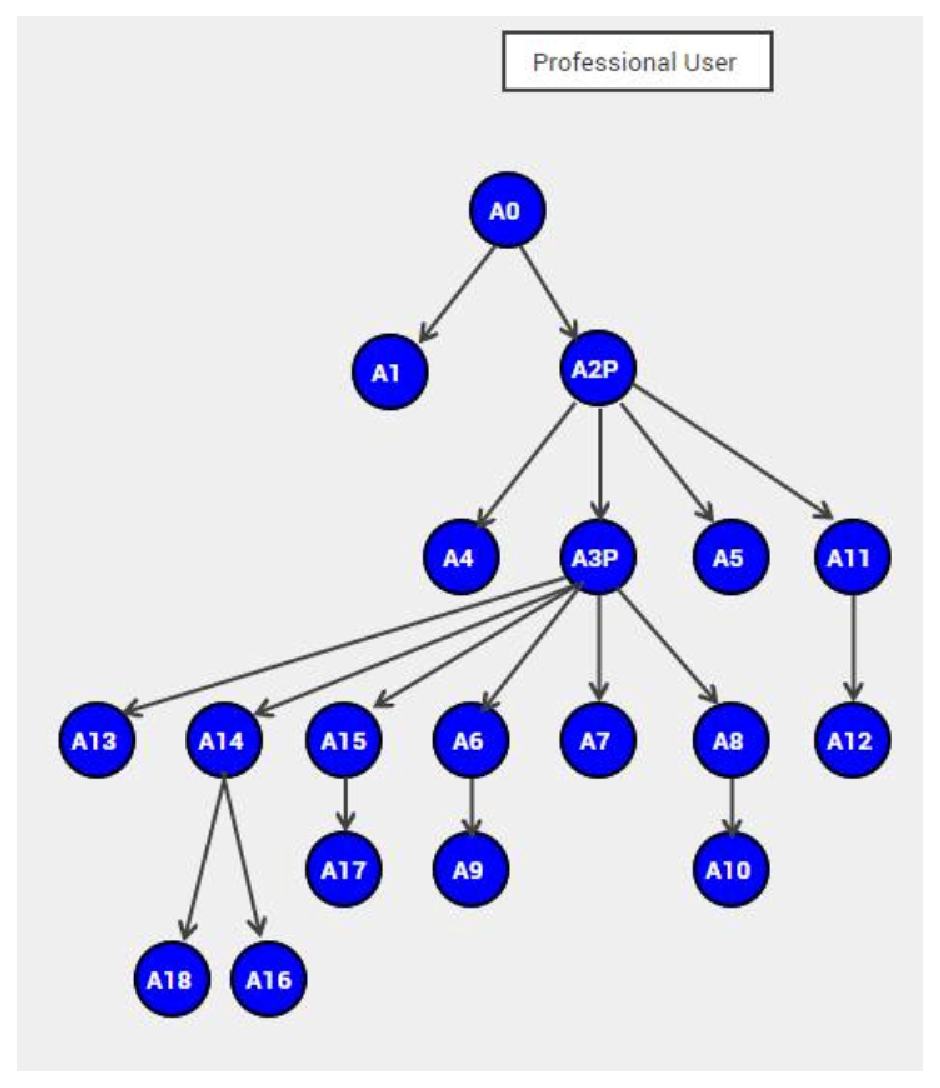
\includegraphics{images/professionaluser.eps}}
\begin{figure}[htbp]
\begin{center}
 \caption{\label{fig:A0} Login Screen}
   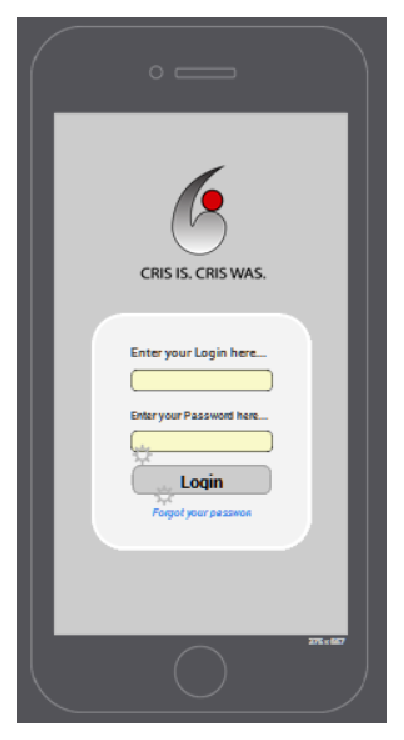
\includegraphics[width=50mm]{./images/App/login.eps}
\end{center}
\end{figure}
\begin{figure}[htbp]
\begin{center}
 \caption{\label{fig:A1} Forgot Password Screen}
   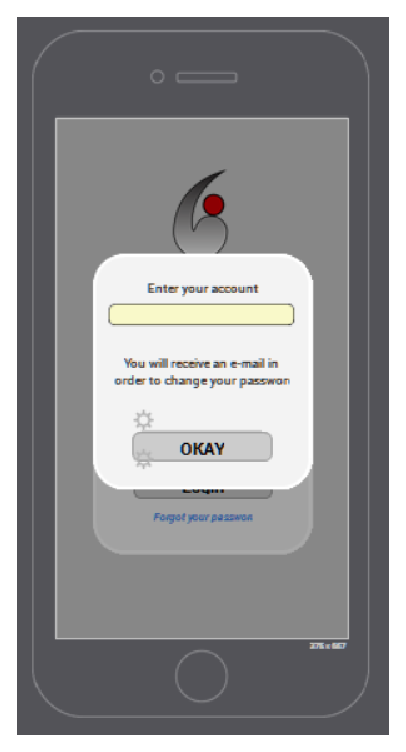
\includegraphics[width=50mm]{./images/App/forgotpasswort.eps}
\end{center}
\end{figure}
\begin{figure}[htbp]
\begin{center}
 \caption{\label{fig:A2P} Home Screen}
   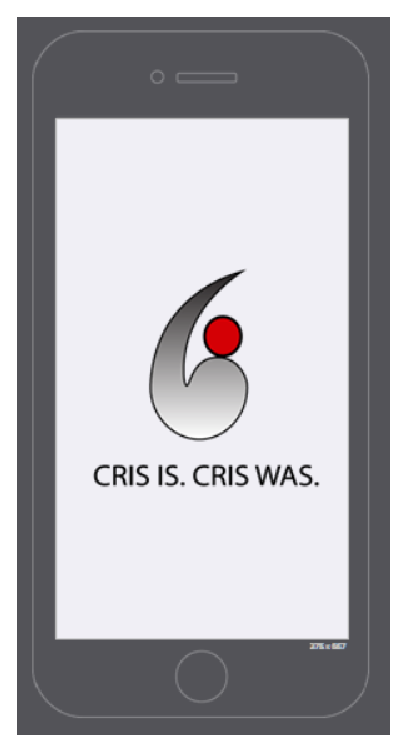
\includegraphics[width=50mm]{./images/App/home.eps}
\end{center}
\end{figure}
\begin{figure}[htbp]
\begin{center}
 \caption{\label{fig:A4} Alert Screen}
   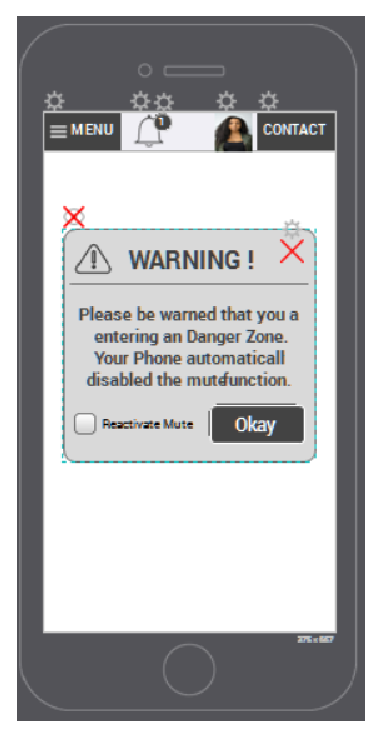
\includegraphics[width=50mm]{./images/App/alerscreen.eps}
\end{center}
\end{figure}
\begin{figure}[htbp]
\begin{center}
 \caption{\label{fig:A3P} Menu Screen}
   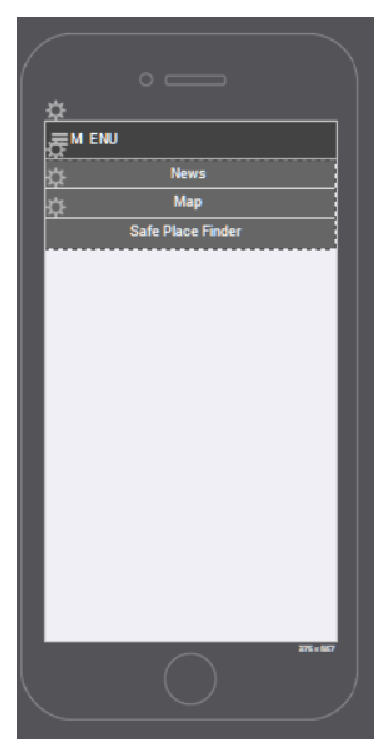
\includegraphics[width=50mm]{./images/App/cmenu.eps}
\end{center}
\end{figure}
\begin{figure}[htbp]
\begin{center}
 \caption{\label{fig:A5} Contact Screen}
   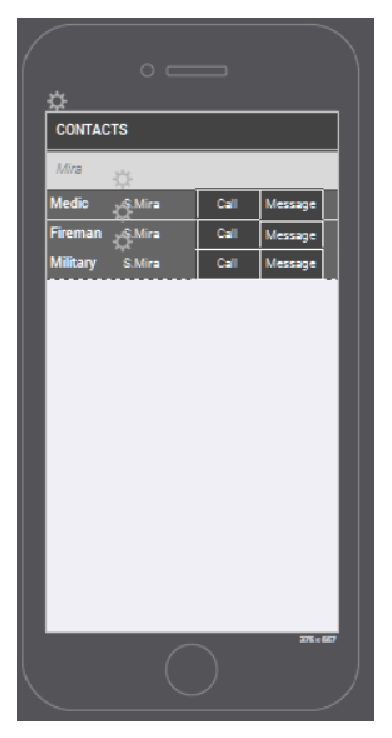
\includegraphics[width=50mm]{./images/App/contactscreen.eps}
\end{center}
\end{figure}
\begin{figure}[htbp]
\begin{center}
 \caption{\label{fig:A11} Account Screen}
   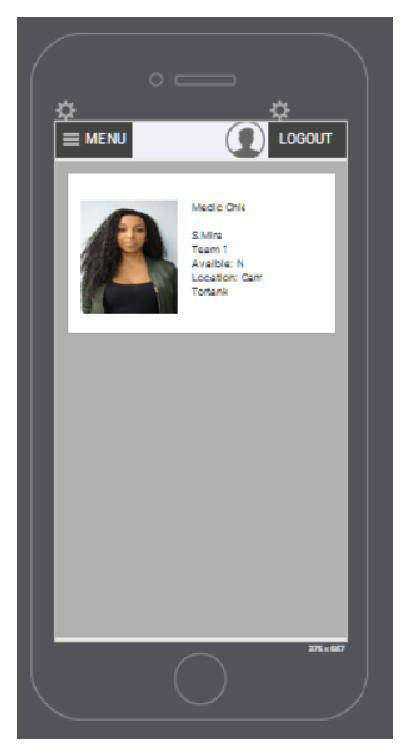
\includegraphics[width=50mm]{./images/App/accountscreen.eps}
\end{center}
\end{figure}
\begin{figure}[htbp]
\begin{center}
 \caption{\label{fig:A13} Start Mission Screen}
   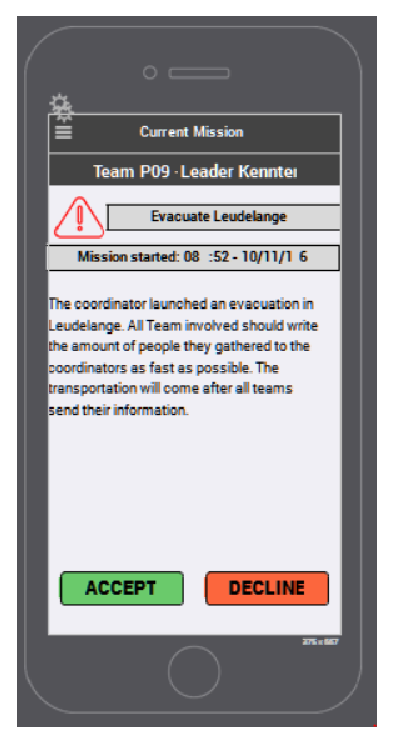
\includegraphics[width=50mm]{./images/App/startmission.eps}
\end{center}
\end{figure}
\begin{figure}[htbp]
\begin{center}
 \caption{\label{fig:A14} Mission Screen}
   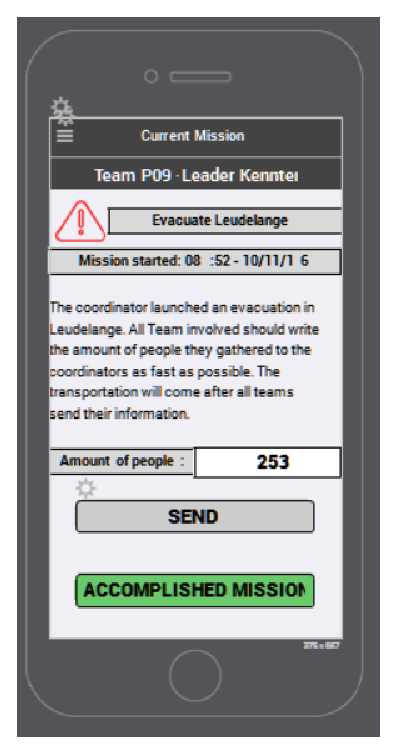
\includegraphics[width=50mm]{./images/App/missionscreen.eps}
\end{center}
\end{figure}
\begin{figure}[htbp]
\begin{center}
 \caption{\label{fig:A15} New Request Screen}
   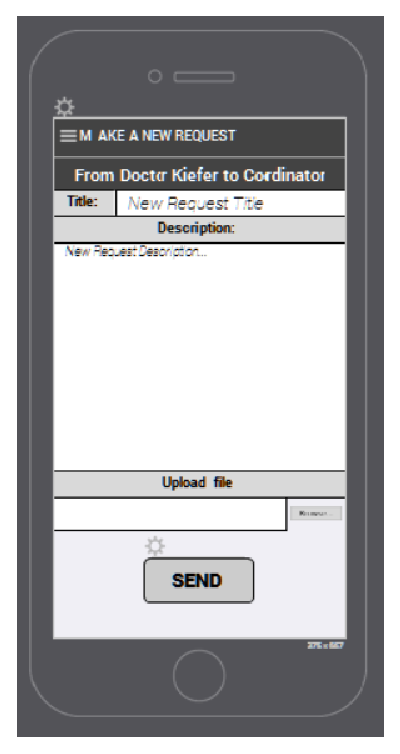
\includegraphics[width=50mm]{./images/App/newrequest.eps}
\end{center}
\end{figure}
\begin{figure}[htbp]
\begin{center}
 \caption{\label{fig:A6} News Screen}
   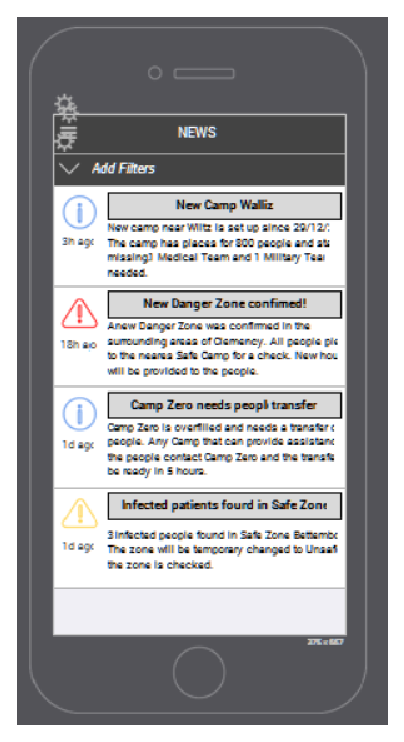
\includegraphics[width=50mm]{./images/App/newsscreen.eps}
\end{center}
\end{figure}
\begin{figure}[htbp]
\begin{center}
 \caption{\label{fig:A7} Map Screen}
   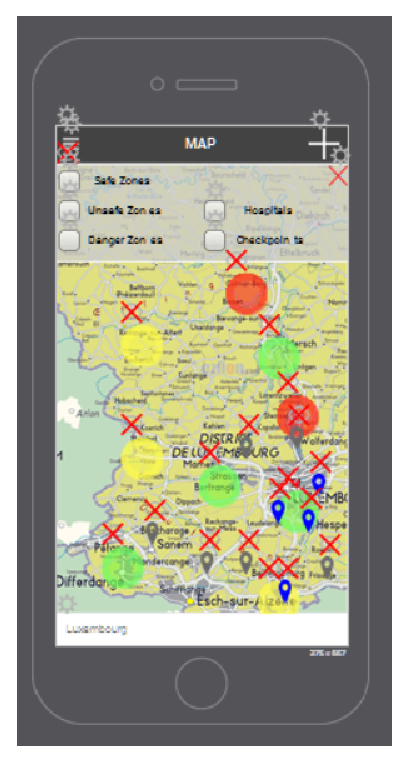
\includegraphics[width=50mm]{./images/App/mapscreen.eps}
\end{center}
\end{figure}
\begin{figure}[htbp]
\begin{center}
 \caption{\label{fig:A8} Safe Place Finder Screen}
   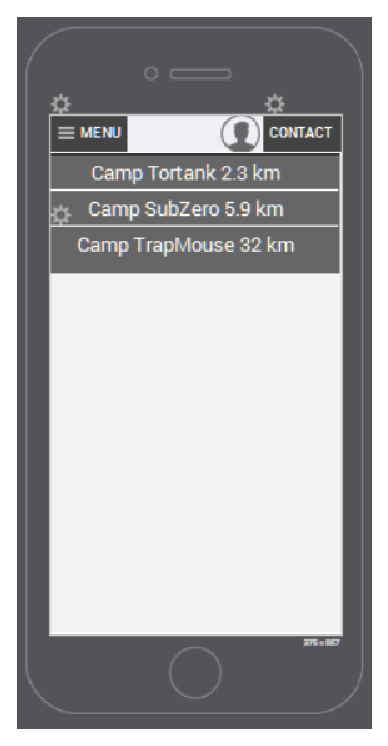
\includegraphics[width=50mm]{./images/App/placefinder.eps}
\end{center}
\end{figure}
\begin{figure}[htbp]
\begin{center}
 \caption{\label{fig:A12} Logout Screen}
   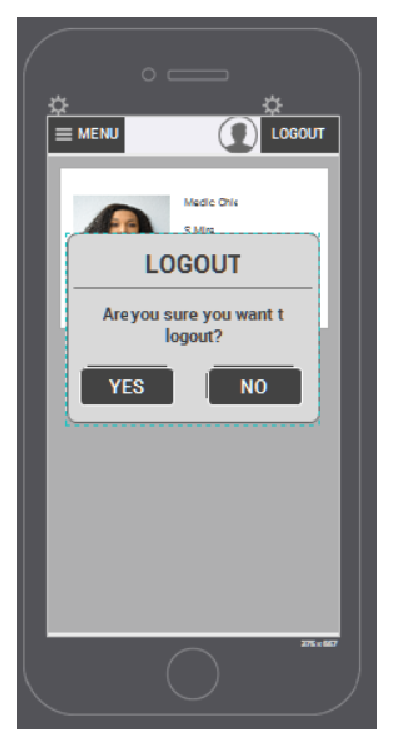
\includegraphics[width=50mm]{./images/App/logoutscreen.eps}
\end{center}
\end{figure}
\begin{figure}[htbp]
\begin{center}
 \caption{\label{fig:A18} Team View Screen}
   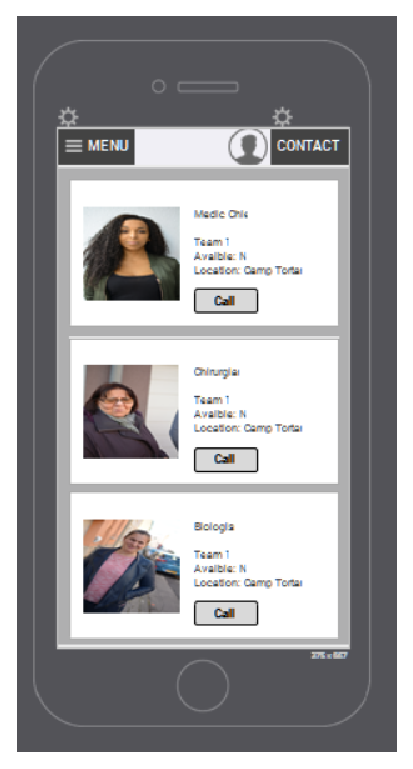
\includegraphics[width=50mm]{./images/App/teamview.eps}
\end{center}
\end{figure}
\begin{figure}[htbp]
\begin{center}
 \caption{\label{fig:A16} Mission Sended Screen}
   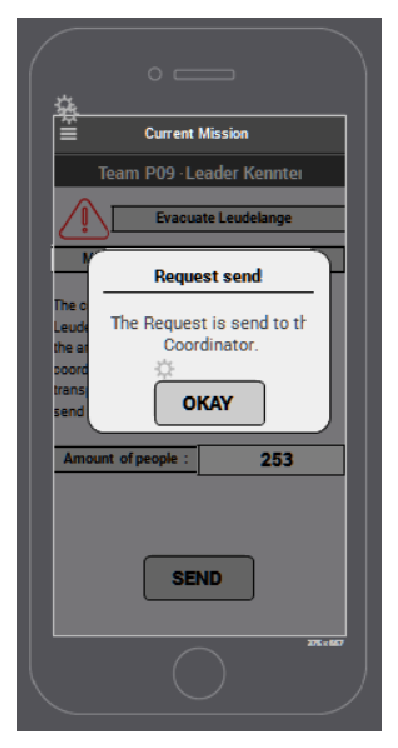
\includegraphics[width=50mm]{./images/App/missionsendedscreen.eps}
\end{center}
\end{figure}
\begin{figure}[htbp]
\begin{center}
 \caption{\label{fig:A17} New Resquest Sended Screen}
   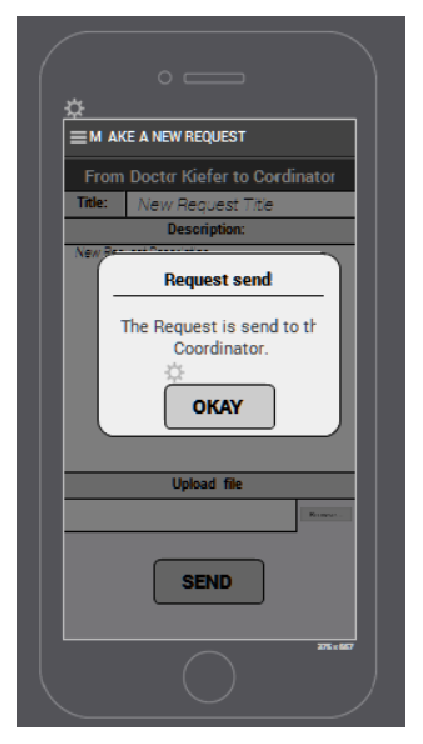
\includegraphics[width=50mm]{./images/App/requstsendedconfirm.eps}
\end{center}
\end{figure}
\begin{figure}[htbp]
\begin{center}
 \caption{\label{fig:A9} News Screen Filter Screen}
   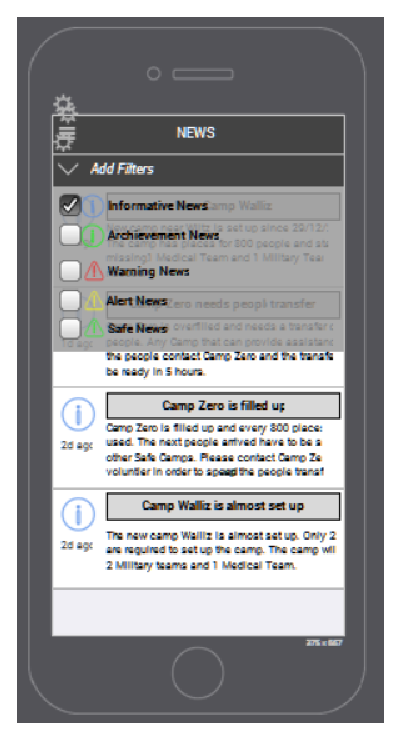
\includegraphics[width=50mm]{./images/App/newsfilter.eps}
\end{center}
\end{figure}
\begin{figure}[htbp]
\begin{center}
 \caption{\label{fig:A10} Trace Screen}
   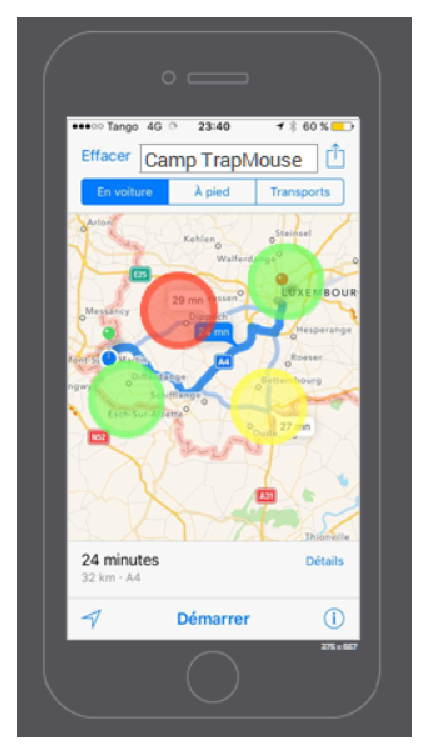
\includegraphics[width=50mm]{./images/App/traceroute.eps}
\end{center}
\end{figure}



\subsection{Web Screens}
\subsubsection{Administrator}
\center{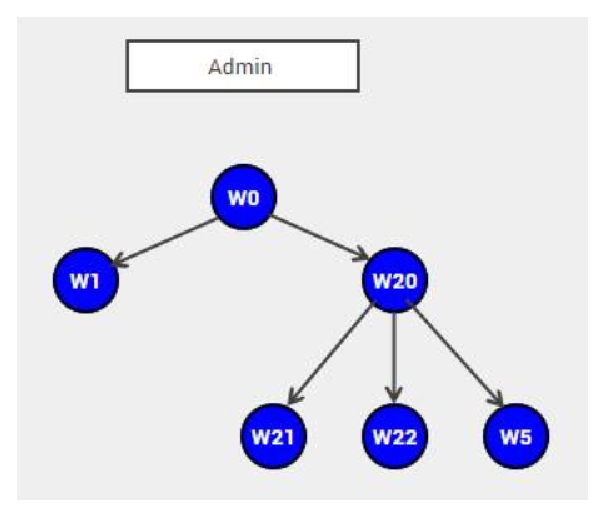
\includegraphics{images/admin.eps}}
\begin{figure}[htbp]
\begin{center}
 \caption{\label{fig:W0} Login Screen}
   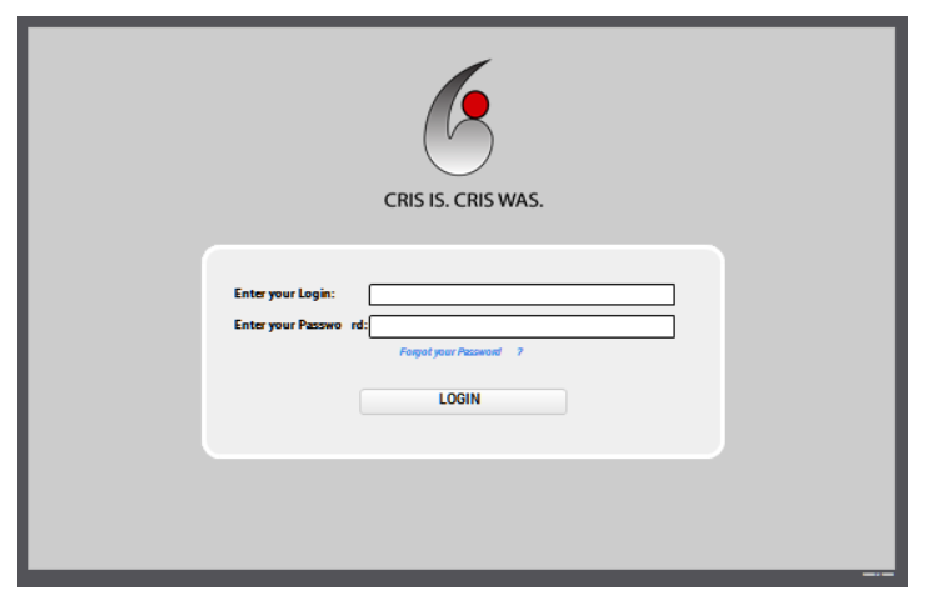
\includegraphics[width=150mm]{./images/Web/login.eps}
\end{center}
\end{figure}
\begin{figure}[htbp]
\begin{center}
 \caption{\label{fig:W1} Forgot Password Screen}
   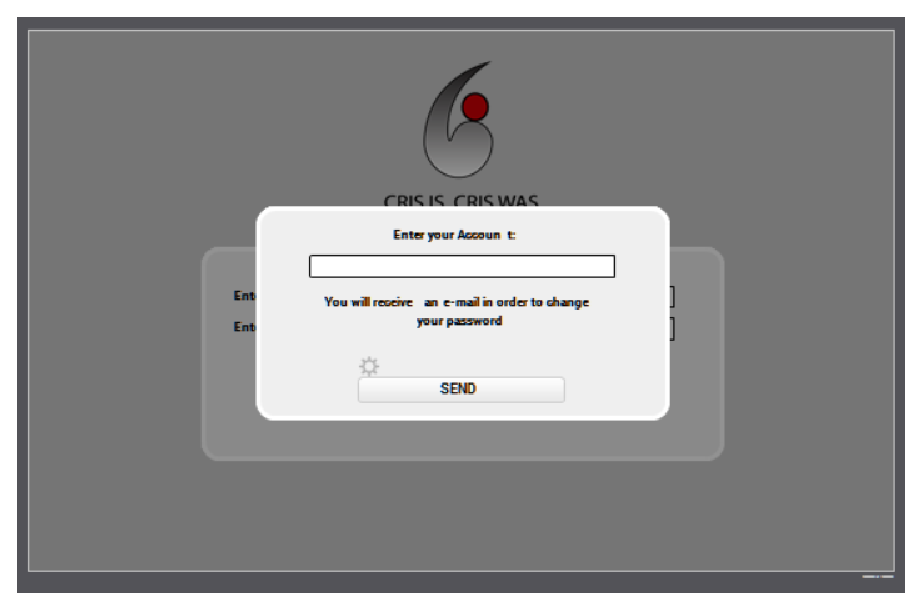
\includegraphics[width=150mm]{./images/Web/forgot.eps}
\end{center}
\end{figure}
\begin{figure}[htbp]
\begin{center}
 \caption{\label{fig:W20} Administrator Main Screen}
   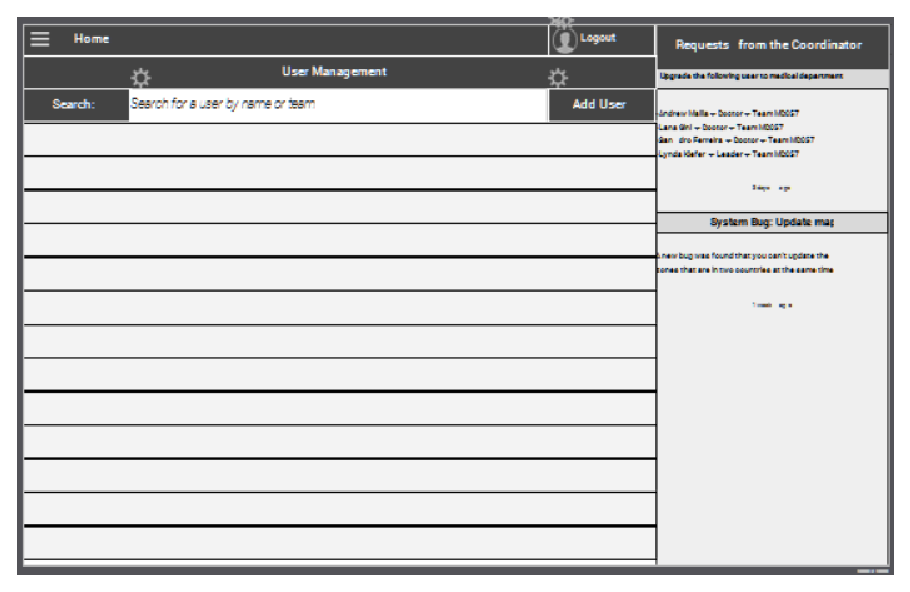
\includegraphics[width=150mm]{./images/Web/aadminmainscreen.eps}
\end{center}
\end{figure}
\begin{figure}[htbp]
\begin{center}
 \caption{\label{fig:W21} Administrator Add Screen}
   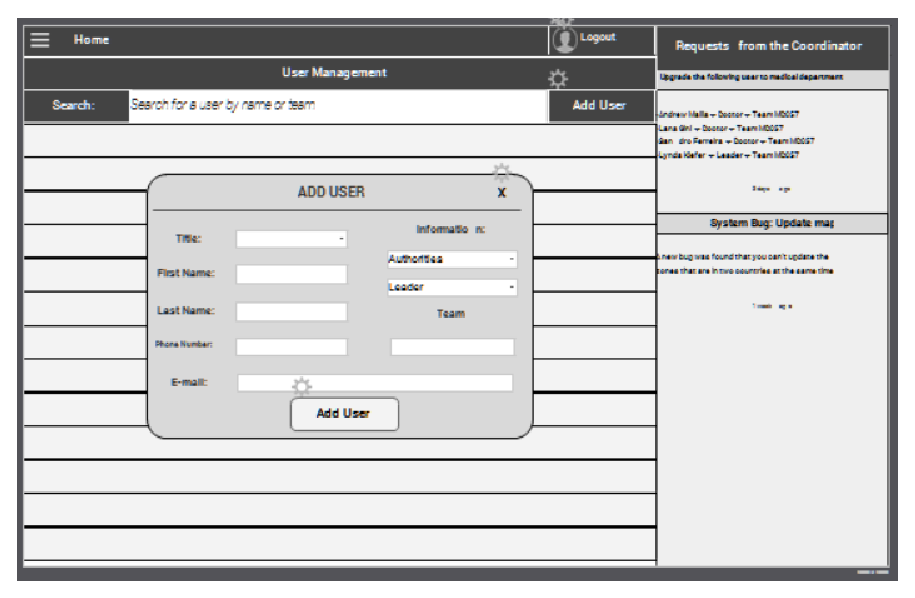
\includegraphics[width=150mm]{./images/Web/aadminaddscreenau.eps}
\end{center}
\end{figure}
\begin{figure}[htbp]
\begin{center}
 \caption{\label{fig:W22} Administrator Update Screen}
   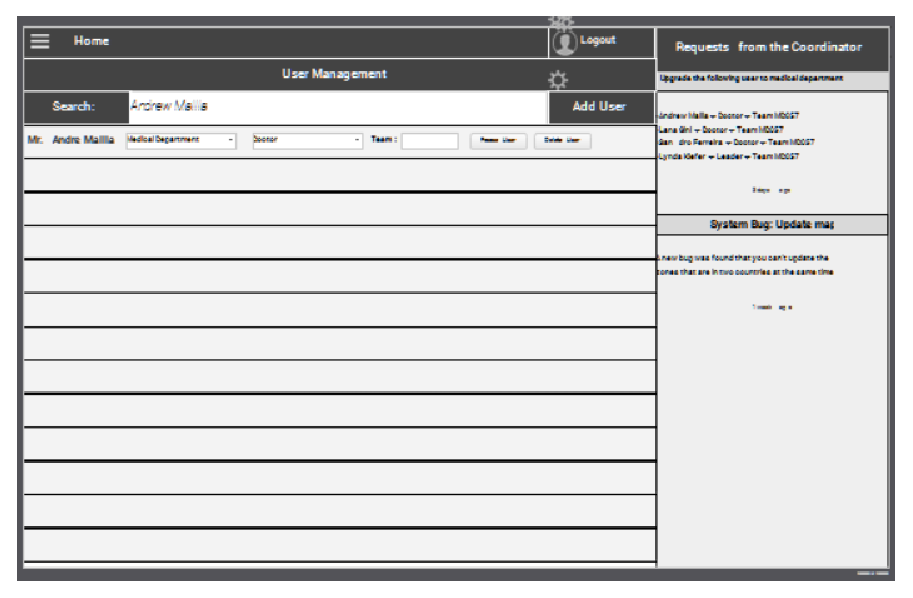
\includegraphics[width=150mm]{./images/Web/adminupdatescreen.eps}
\end{center}
\end{figure}
\begin{figure}[htbp]
\begin{center}
 \caption{\label{fig:W5} Logout Screen}
   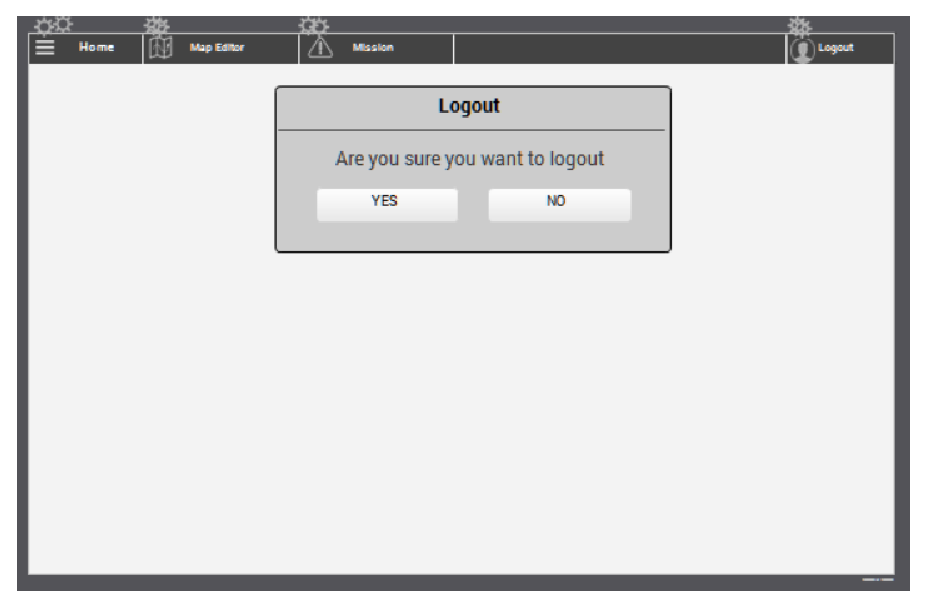
\includegraphics[width=150mm]{./images/Web/logout.eps}
\end{center}
\end{figure}



\subsubsection{Coordinator}
\center{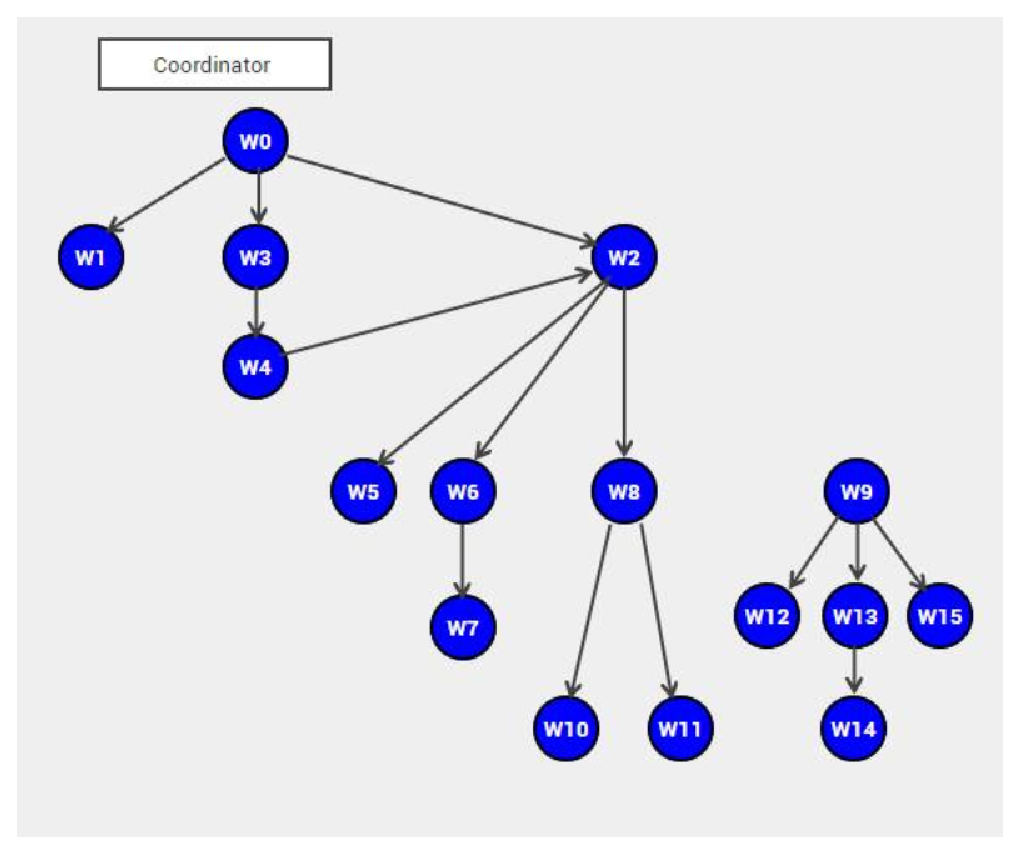
\includegraphics{images/coordinator.eps}}
\begin{figure}[htbp]
\begin{center}
 \caption{\label{fig:W0} Login Screen}
   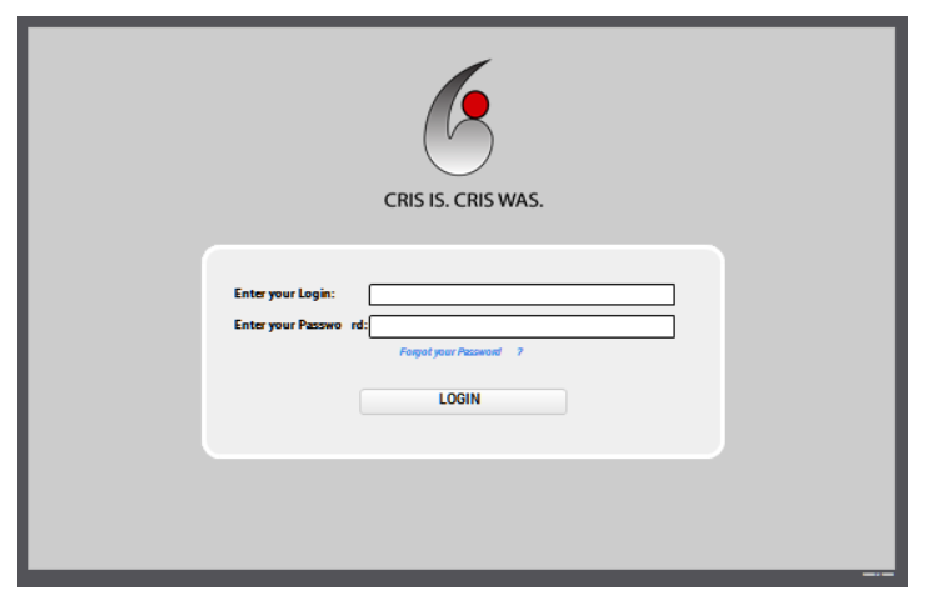
\includegraphics[width=150mm]{./images/Web/login.eps}
\end{center}
\end{figure}
\begin{figure}[htbp]
\begin{center}
 \caption{\label{fig:W1} Forgot Password Screen}
   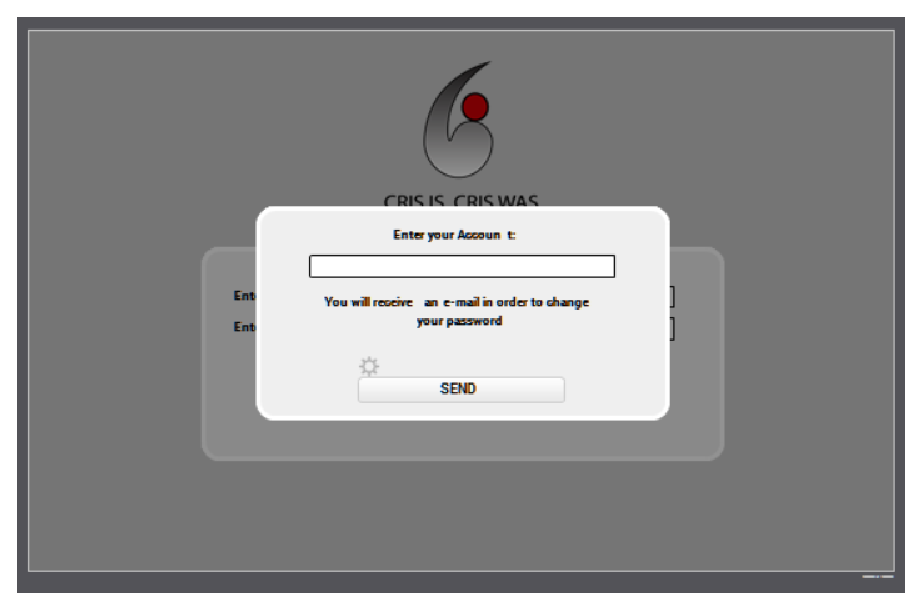
\includegraphics[width=150mm]{./images/Web/forgot.eps}
\end{center}
\end{figure}
\begin{figure}[htbp]
\begin{center}
 \caption{\label{fig:W3} Get Alert Screen}
   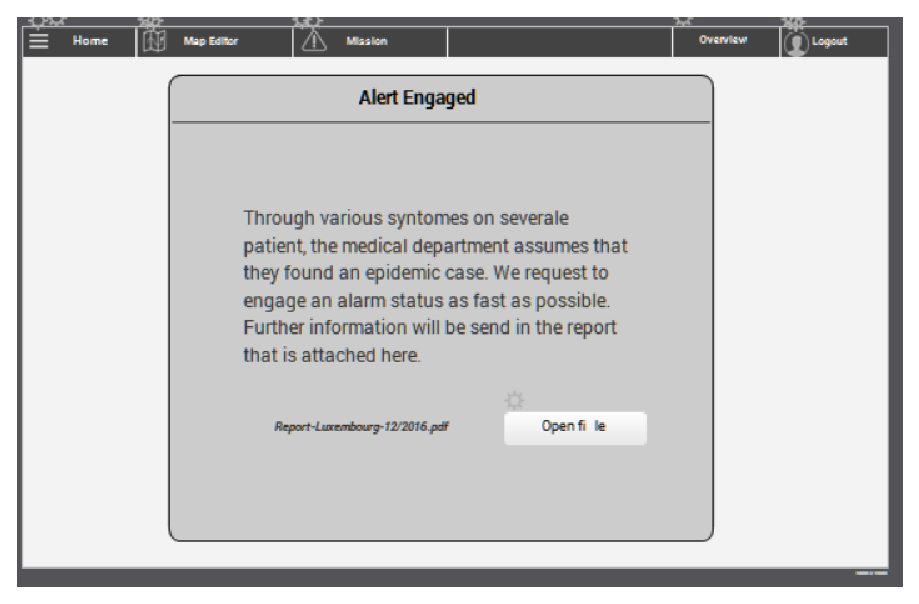
\includegraphics[width=150mm]{./images/Web/cgetalert.eps}
\end{center}
\end{figure}
\begin{figure}[htbp]
\begin{center}
 \caption{\label{fig:W2} Home Screen}
   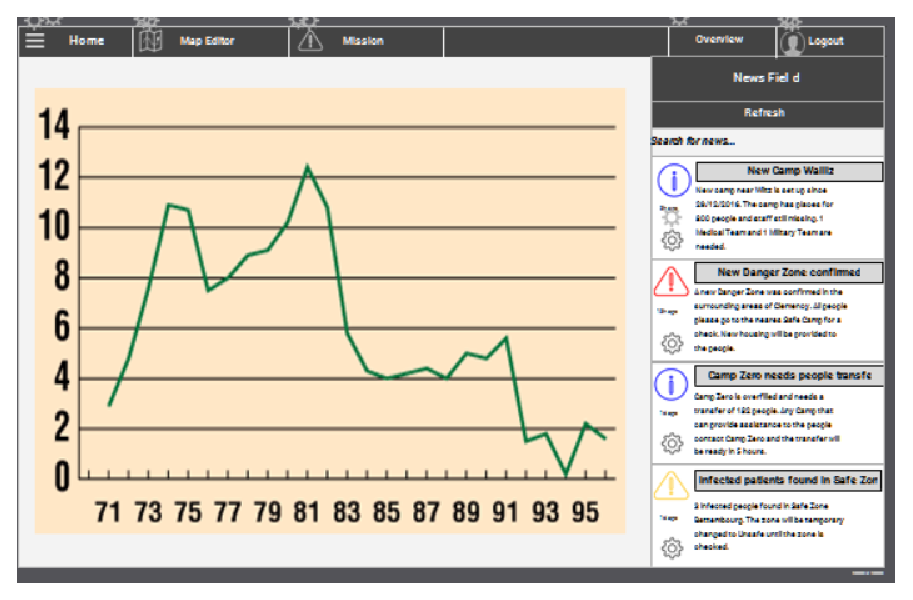
\includegraphics[width=150mm]{./images/Web/chomescreen.eps}
\end{center}
\end{figure}
\begin{figure}[htbp]
\begin{center}
 \caption{\label{fig:We16} Lift Alert}
   \includegraphics[width=150mm]{./images/Web/liftalert1.eps}
\end{center}
\end{figure}
\begin{figure}[htbp]
\begin{center}
 \caption{\label{fig:We17} Lift Alert Confirmation}
   \includegraphics[width=150mm]{./images/Web/alertlift.eps}
\end{center}
\end{figure}
\begin{figure}[htbp]
\begin{center}
 \caption{\label{fig:W4} Report Screen}
   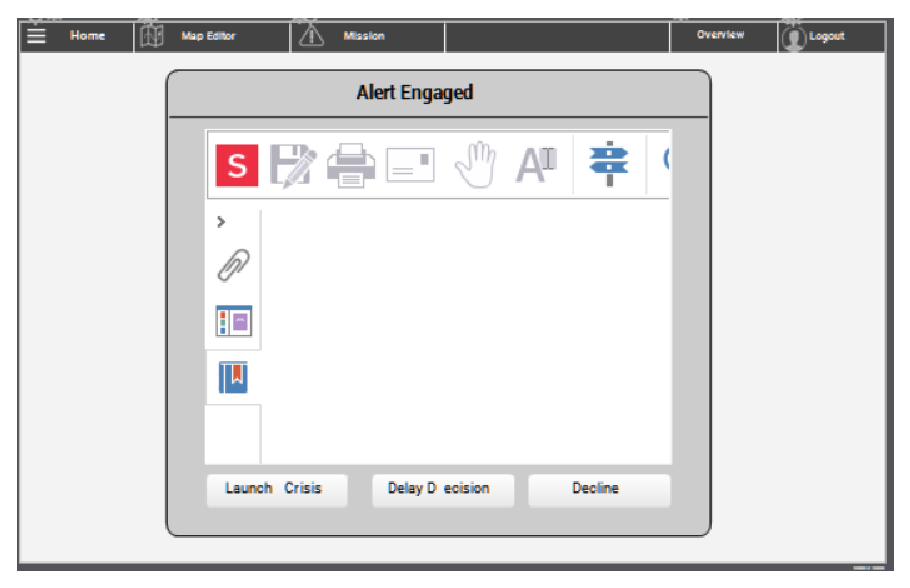
\includegraphics[width=150mm]{./images/Web/calertengaged.eps}
\end{center}
\end{figure}
\begin{figure}[htbp]
\begin{center}
 \caption{\label{fig:W5} Logout Screen}
   \includegraphics[width=150mm]{./images/Web/logout.eps}
\end{center}
\end{figure}
\begin{figure}[htbp]
\begin{center}
 \caption{\label{fig:W6} Overview 1 Screen}
   \includegraphics[width=150mm]{./images/Web/coverview2.eps}
\end{center}
\end{figure}
\begin{figure}[htbp]
\begin{center}
 \caption{\label{fig:W8} Mission Screen}
   \includegraphics[width=150mm]{./images/Web/cmissionscreen.eps}
\end{center}
\end{figure}
\begin{figure}[htbp]
\begin{center}
 \caption{\label{fig:W7} Overview 2 Screen}
   \includegraphics[width=150mm]{./images/Web/coverview3.eps}
\end{center}
\end{figure}
\begin{figure}[htbp]
\begin{center}
 \caption{\label{fig:W10} Add Zone Screen}
   \includegraphics[width=150mm]{./images/Web/addzone.eps}
\end{center}
\end{figure}
\begin{figure}[htbp]
\begin{center}
 \caption{\label{fig:W11} Set Zone Screen}
   \includegraphics[width=150mm]{./images/Web/setzone.eps}
\end{center}
\end{figure}
\begin{figure}[htbp]
\begin{center}
 \caption{\label{fig:W9} Map Screen}
   \includegraphics[width=150mm]{./images/Web/map.eps}
\end{center}
\end{figure}
\begin{figure}[htbp]
\begin{center}
 \caption{\label{fig:W12} Mission Send Screen}
   \includegraphics[width=150mm]{./images/Web/cmissionsendscreen.eps}
\end{center}
\end{figure}
\begin{figure}[htbp]
\begin{center}
 \caption{\label{fig:W13} Setting Mission Screen}
   \includegraphics[width=150mm]{./images/Web/csettingmissionscreen.eps}
\end{center}
\end{figure}
\begin{figure}[htbp]
\begin{center}
 \caption{\label{fig:W15} Setting Chackpoint Screen}
   \includegraphics[width=150mm]{./images/Web/ccheckpointsc.eps}
\end{center}
\end{figure}
\begin{figure}[htbp]
\begin{center}
 \caption{\label{fig:W14} Mission Update Screen}
   \includegraphics[width=150mm]{./images/Web/cupdatescreen.eps}
\end{center}
\end{figure}


\section{Error Warnings}
\label{sec:ErrorWarnings}

\begin{figure}[htbp]
\begin{center}
 \caption{\label{fig:E1} Access Denied}
   \includegraphics[width=50mm]{./images/Errors/accessdenied.eps}
\end{center}
\end{figure}

\begin{figure}[htbp] 
\begin{center}
 \caption{\label{fig:E2} Internet Connection Missing}
   \includegraphics[width=50mm]{./images/Errors/internetcon.eps}
\end{center}
\end{figure}

\begin{figure}[htbp]
\begin{center}
 \caption{\label{fig:E3} Mobile Connection Missing}
   \includegraphics[width=50mm]{./images/Errors/mobilenetwork.eps}
\end{center}
\end{figure}

\begin{figure}[htbp]
\begin{center}
 \caption{\label{fig:E4} Server Crash}
   \includegraphics[width=50mm]{./images/Errors/servercrash.eps}
\end{center}
\end{figure}
 

	

\newpage

   
%GLOSSARY
%Uncomment the line below if you want to print all glossaries no matter if they
% appear in the document
%\glsaddall
\printglossaries
\newpage


%BIBLIOGRAPHY
\cleardoublepage 
\bibliographystyle{./../lu.uni.lassy.excalibur.standard.report.libraries/styles/lncs} 
\bibliography{./../lu.uni.lassy.excalibur.standard.report.libraries/defs/references/messir,doc/bibliography/user-manual}
\label{sec:references}

 
\end{document}
